\documentclass{book}
\usepackage[english]{babel}     
\usepackage[utf8]{inputenc}     % accent symbols
\usepackage[T1]{fontenc}
\usepackage{lmodern}
\usepackage{microtype}
\usepackage{natbib}
\usepackage{tocbibind}          
\usepackage{amsmath}            % math symbols
\usepackage{amsthm}             % math symbols
\usepackage[colorlinks=true,linkcolor=red]{hyperref} % hyper link

% for code
\usepackage{listings}
\usepackage{color,xcolor}
\definecolor{mygreen}{rgb}{0,0.6,0}
\definecolor{mygray}{rgb}{0.9,0.9,0.9}
\definecolor{mymauve}{rgb}{0.58,0,0.82}
\lstset{
backgroundcolor=\color{mygray},
numbers=left,                    
columns=fullflexible,
breaklines=true,      
captionpos=b,         
tabsize=4,            
commentstyle=\color{mygreen}, 
escapeinside={\%*}{*)},       
keywordstyle=\color{blue},    
% stringstyle=\color{mymauve}\monaco,
frame=single,                        
rulesepcolor=\color{red!20!green!20!blue!20},
% identifierstyle=\color{red},
%% language=c++,
basicstyle=\tiny
}

\usepackage{indentfirst}
\setlength{\parindent}{2em}
\usepackage[onehalfspacing]{setspace}
% graph
\usepackage{pdfpages}
\usepackage{graphicx}
% box
\usepackage{booktabs}
\usepackage{tcolorbox}

%% user defined command
\newcommand{\keyword}[1]{\textbf{#1}}
\newcommand{\keywords}[1]{\textbf{#1}}
\newcommand{\lcmd}[1]{\texttt{#1}}
\newcommand{\head}[1]{\textnormal{\textbf{#1}}}
\newcommand{\itwords}[1]{\textit{#1}}

\usepackage{float}
% all symbols
\usepackage{tipa}
\usepackage{tipx}

\usepackage{datetime}
% \usepackage{movie15}


% variable
% TODO
\newcommand{\pdfauthor}{Mike Chyson (Li Mingming)}
\newcommand{\pdftitle}{Principles of Economics}
\newcommand{\pdfsubject}{Principles of Economics}
\newcommand{\pdfkeywords}{Principles of Economics}
\newcommand{\bookname}{Principles of Economics}
\newcommand{\bookoneword}{Citation and interpreation of principles of economics}
\newcommand{\timeandcompany}{Dec, 5, 2020}

\usepackage{bm}
\usepackage{amsfonts}
\hypersetup{
  pdfauthor={\pdfauthor},   
  pdftitle={\pdftitle},     
  pdfsubject={\pdfsubject}, 
  pdfkeywords={\pdfkeywords}
}
% \includeonly{}
\begin{document}
\frontmatter
\begin{titlepage}
  \raggedleft
      {\Large 作者\\ 李明明\\[1in] }
  % {\large 关于\\}
  {\Huge\scshape 法语学习\\[.2in]}
  {\large 从零学习法语的笔记整理 \\}
  \vfill
  {\itshape \today{}}
\end{titlepage}


\chapter*{Dedication}

读《经济学原理》的笔记。


\mainmatter
\tableofcontents



\chapter{Ten principles of economics}


The word economy comes from the Greek word for ``one who manages a household.''
Economics is the study of how society manages its scarce resources.

\section{How people make decisions}

\subsection*{PRINCIPLE 1: PEOPLE FACE TRADEOFFS}

To get one thing that we like, we usually have to give up another thing that we like.
Making decisions requires trading off one goal against another.


\subsection*{PRINCIPLE 2: THE COST OF SOMETHING IS WHAT YOU GIVE UP TO GET IT}

Because people face tradeoffs, making decisions requires comparing the costs and benefits of alternative courses of action.
The opportunity cost of an item is what you give up to get that item.

\subsection*{PRINCIPLE 3: RATIONAL PEOPLE THINK AT THE MARGIN}

Economists use the term marginal changes to describe small incremental adjustments to an existing plan of action.
Keep in mind that ``margin'' means ``edge,'' so marginal changes are adjustments around the edges of what you are doing.

\subsection*{PRINCIPLE 4: PEOPLE RESPOND TO INCENTIVES}

Because people make decisions by comparing costs and benefits, their behavior may change when the costs or benefits change.
That is, people respond to incentives. 

\section{How people interact}

\subsection*{PRINCIPLE 5: TRADE CAN MAKE EVERYONE BETTER OFF}

Trade allows each person to specialize in the activities he or she does best, whether it is farming, sewing, or home building.
By trading with others, people can buy a greater variety of goods and services at lower cost.
Countries as well as families benefit from the ability to trade with one another.
Trade allows countries to specialize in what they do best and to enjoy a greater variety of goods and services.

\begin{tcolorbox}
  Thus, it is import to decide what you want to \emph{specialize} in.
\end{tcolorbox}


\subsection*{PRINCIPLE 6: MARKETS ARE USUALLY A GOOD WAY TO ORGANIZE ECONOMIC ACTIVITY}

In a market economy, the decisions of a central planner are replaced by the decisions of millions of firms and households.
Firms decide whom to hire and what to make.
Households decide which firms to work for and what to buy with their incomes.
These firms and households interact in the marketplace, where prices and self-interest guide their decisions.

In his 1776 book \emph{An Inquiry into the Nature and Causes of the Wealth of Nations}, economist Adam Smith made the most famous observation in all of economics: Households and firms interacting in markets act as if they are guided by an ``invisible hand'' that leads them to desirable market outcomes.

Prices are the instrument with which the invisible hand directs economic activity.
Prices reflect both the value of a good to society and the cost to society of making the good.
Because households and firms look at prices when deciding what to buy and sell, they unknowingly take into account the social benefits and costs of their actions.
As a result, prices guide these individual decisionmakers to reach outcomes that, in many cases, maximize the welfare of society as a whole.

\subsection*{PRINCIPLE 7: GOVERNMENTS CAN SOMETIMES IMPROVE MARKET OUTCOMES}

Although markets are usually a good way to organize economic activity, this rule has some important exceptions.
There are two broad reasons for a government to intervene in the economy: to promote efficiency and to promote equity.
That is, most policies aim either to enlarge the economic pie or to change how the pie is divided.



The invisible hand usually leads markets to allocate resources efficiently.
Nonetheless, for various reasons, the invisible hand sometimes does not work.
Economists use the term \emph{market failure} to refer to a situation in which the market on its own fails to allocate resources efficiently.



One possible cause of market failure is an \emph{externality}.
An externality is the im- pact of one person’s actions on the well-being of a bystander.
Another possible cause of market failure is \emph{market power}.
Market power refers to the ability of a single person (or small group of people) to unduly influence market prices.


\section{How the econmy as a whole works}

\subsection*{PRINCIPLE 8: A COUNTRY’S STANDARD OF LIVING DEPENDS ON ITS ABILITY TO PRODUCE GOODS AND SERVICES}

\subsection*{PRINCIPLE 9: PRICES RISE WHEN THE GOVERNMENT PRINTS TOO MUCH MONEY}

What causes inflation? In almost all cases of large or persistent inflation, the culprit turns out to be the same—growth in the quantity of money.
When a government creates large quantities of the nation’s money, the value of the money falls.



\subsection*{PRINCIPLE 10: SOCIETY FACES A SHORT-RUN TRADEOFF BETWEEN INFLATION AND UNEMPLOYMENT}

If inflation is so easy to explain, why do policymakers sometimes have trouble ridding the economy of it?
One reason is that reducing inflation is often thought to cause a temporary rise in unemployment.
The curve that illustrates this tradeoff between inflation and unemployment is called the Phillips curve, after the economist who first examined this relationship.


Why do we face this short-run tradeoff?
According to a common explanation, it arises because some prices are slow to adjust.
Suppose, for example, that the government reduces the quantity of money in the economy.
In the long run, the only result of this policy change will be a fall in the overall level of prices.
Yet not all prices will adjust immediately.
It may take several years before all firms issue new catalogs, all unions make wage concessions, and all restaurants print new menus.
That is, prices are said to be sticky in the short run.


Because prices are sticky, various types of government policy have short-run effects that differ from their long-run effects.
When the government reduces the quantity of money, for instance, it reduces the amount that people spend.
Lower spending, together with prices that are stuck too high, reduces the quantity of goods and services that firms sell.
Lower sales, in turn, cause firms to lay off workers.
Thus, the reduction in the quantity of money raises unemployment temporarily until prices have fully adjusted to the change.





\chapter{Thinking like an economist}

Every field of study has its own language and its own way of thinking.
The most important is to learn the economist's of thinking.


\section{The economist as scientist}

Economist try to address their subject with a scientist's objectivity:
\begin{itemize}
\item devise theories
\item collect data
\item analyze these data in an attempt to verify or refute their theories
\end{itemize}

\begin{tcolorbox}
  The essence of science is the scientific method -- the dispassinate development and testing of theories about how the world works.
\end{tcolorbox}

As Albert Einstein once put it, ``The whole of science is nothing more than the refinement of everyday thinking''.


\subsection{The scientific method}

The scientific method:
\begin{enumerate}
\item observation
\item theory
\item more observation
\end{enumerate}

Although economists use theory and observation like other scientists, they do face an obstacle that makes their task especially challenging: Experiments are often difficult in economics.

\subsection{The role of assumptions}

Assumptions can make the world easier to understand.
The art in scientific thinking is deciding which assumptions to make.
Economists use different assumptions when studying the short-run and long-run efects of a change in the quantity of money.

\subsection{Economic models}

Economists use models that are most often composed of diagrams and equations to learn about the world.
Economic models omit many details to allow us to see what is truely important.
An economist's model does not include every feature of the economy.
All models are built with assumptions.
Economists assume away many of the details of the economy that are errelevant for studying the question at hand.
All models simplify reality in order to improve our understanding of it.

\subsection{The circular-flow diagram}

Circular-flow diagram: a visual model of the economy that shows how dollars flow through markets among households and firms.


\begin{figure}[!ht]
  \centering
  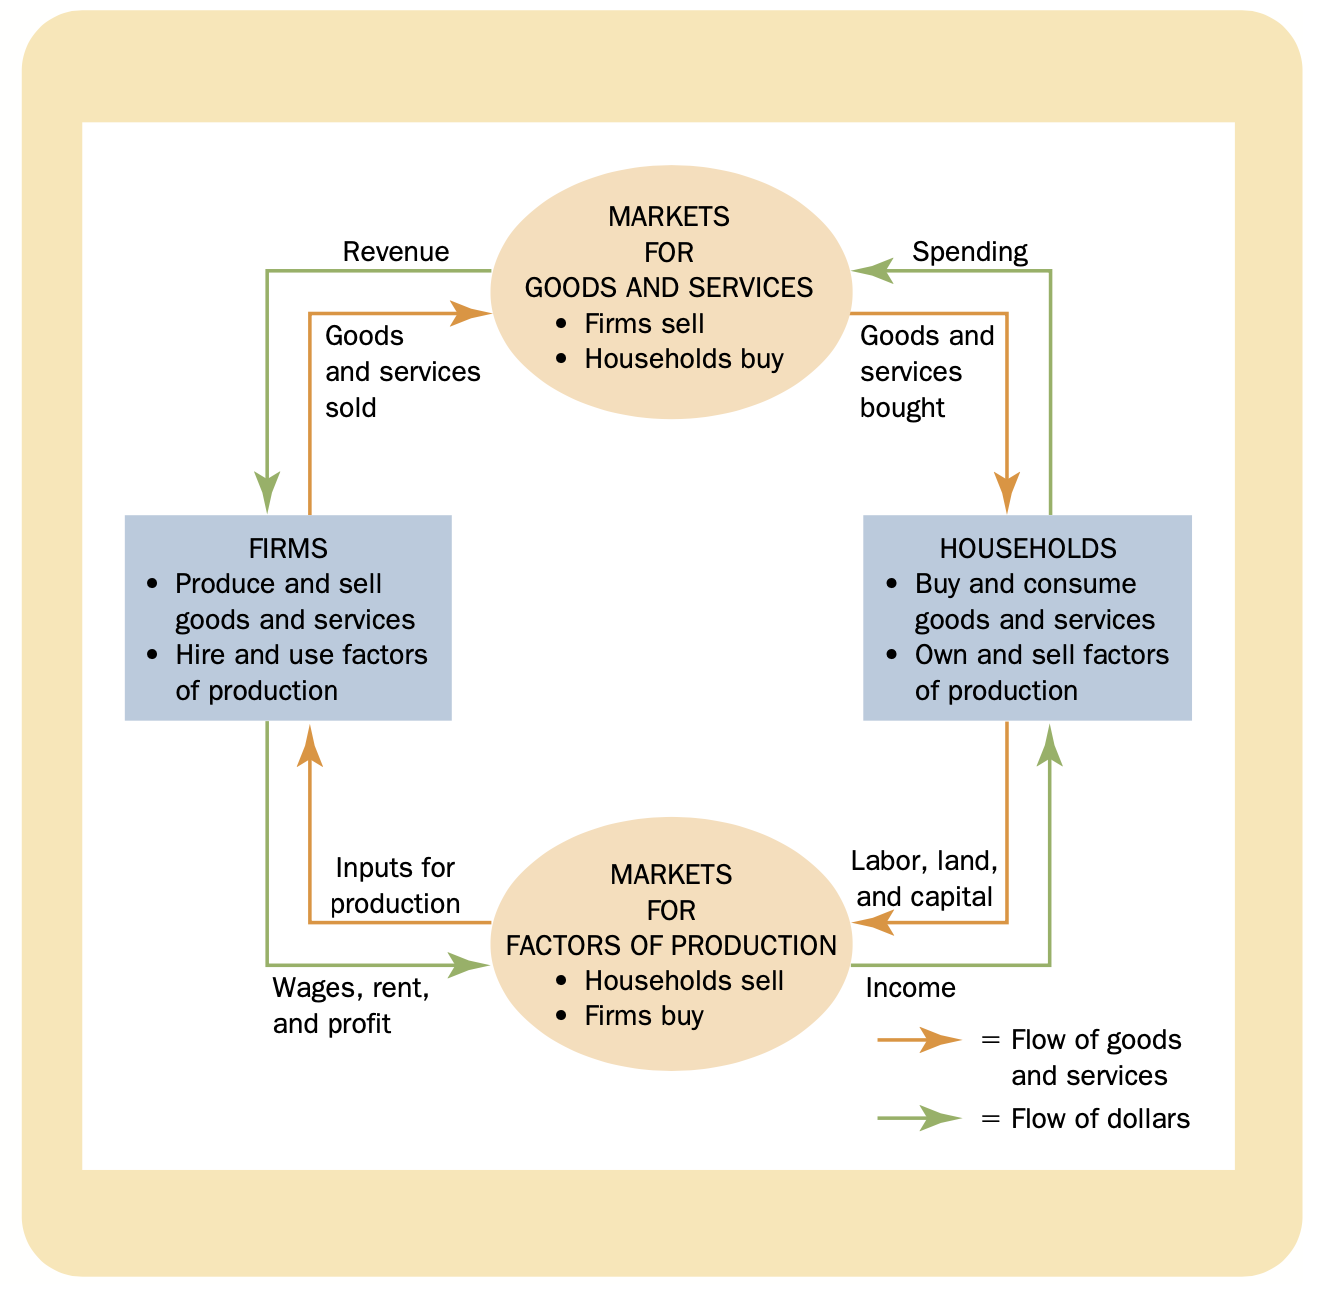
\includegraphics[width=\textwidth]{pics/circular-flow.png}
  \caption{The circular flow}
  \label{fig:circular-flow}
\end{figure}


\subsection{The production possibilities frontier}

Most economics models are built using the tools of mathematics.
Here we consider one of the simplest such models, called the production possibilities frontier.
The \keyword{production possibilities frontier} is a graph that shows the various combinations of output that the economy can possibly produce given the available factors of production and the available production technology that firms can use to turn these factors into output. The graph is shown in Figure \ref{fig:the-production-possibilities-frontier}.



\begin{figure}[!ht]
  \centering
  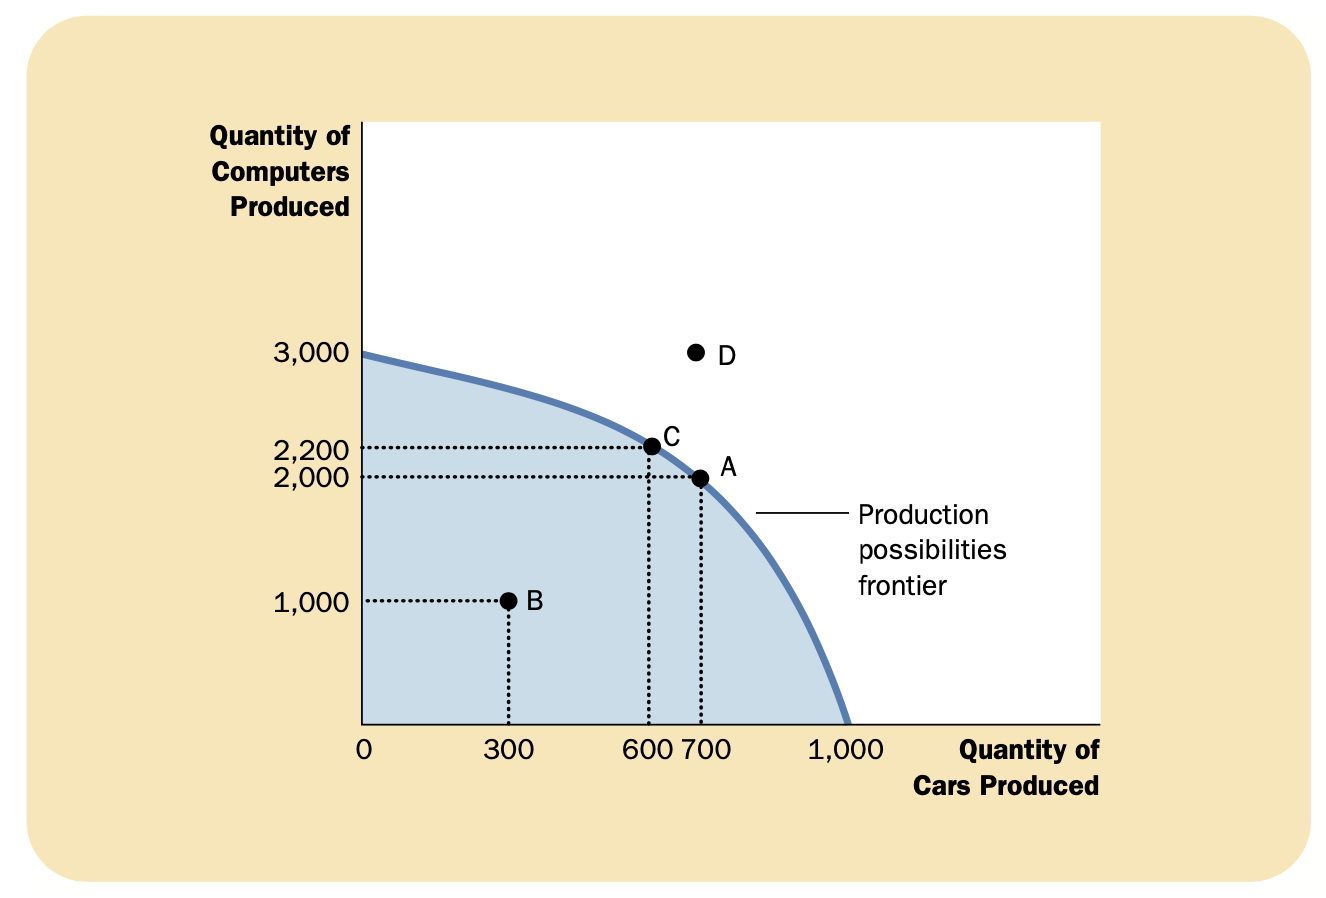
\includegraphics[width=\textwidth]{pics/the-production-possibilities-frontier}
  \caption{The production possibilities frontier}
  \label{fig:the-production-possibilities-frontier}
\end{figure}



An outcome is said to be \keyword{efficient} if the economy is getting all it can from the scarce resources it has available.
Points on (rather than inside) the production possibilities frontier represent efficient levels of production.



\subsection{Microeconomics and macroeconomics}

The field of economics is traditionally divided into two broad subfields.
\keyword{Microeconomics} is the study of how households and firms make decisions and how they interact in specific markets.
\keyword{Macroeconomics} is the study of economywide phenomena.



Microeconomics and macroeconomics are closely intertwined.
Because changes in the overall economy arise from the decisions of millions of individuals, it is impossible to understand macroeconomic developments without considering the associated microeconomic decisions.
Despite the inherent link between microeconomics and macroeconomics, the two fields are distinct.


\section{The economist as policy adviser}


When economists are trying to explain the world, they are \keyword{scientists}.
When they are trying to help improve it, they are \keyword{policy advisers}.


\subsection{Positive versus normative analysis}


Because scientists and policy advisers have different goals, they use language in different ways.
In general, statements about the world are of two types.
One type is positive.
\keyword{Positive statements} are descriptive.
They make a clain about how the world \keyword{is}.
A second type of statement is normative.
\keyword{Normative statements} are are prescrptive.
They make a clain about how the world \keyword{ought to be}.


A key difference between positive and normative statements is how we judge their validity.
We can, in principle, confirm or refute positive statements by exam- ining evidence.
By contrast, evaluating normative statements involves values as well as facts.


Much of economics just tries to explain how the economy works.
Yet often the goal of economics is to improve how the economy works.
When you hear economists making normative statements, you know they have crossed the line from scientist to policy adviser.



\section{Why economists disagree}

Why do economists so often appear to give conflicting advice to policymakers?
There are two basic reasons:
\begin{itemize}
\item Economists may disagree about the validity of alternative positive theories about how the world works.
\item Economists may have different values and, therefore, different normative views about what policy should try to accomplish.
\end{itemize}


Because of differences in scientific judgments and differences in values, some disagreement among economists is inevitable.
Yet one should not overstate the amount of disagreement.
In many cases, economists do offer a united view.


You might find it helpful to keep in mind some advice from the great economist John Maynard Keynes:

\begin{tcolorbox}
The study of economics does not seem to require any specialized gifts of an unusually high order. Is it not \dots a very easy subject compared with the higher branches of philosophy or pure science? An easy subject, at which very few excel! The paradox finds its explanation, perhaps, in that the master-economist must possess a rare combination of gifts. He must be mathematician, historian, statesman, philosopher—in some degree. He must understand symbols and speak in words. He must contemplate the particular in terms of the general, and touch abstract and concrete in the same flight of thought. He must study the present in the light of the past for the purposes of the future. No part of man’s nature or his institutions must lie entirely outside his regard. He must be purposeful and disinterested in a simultaneous mood; as aloof and incorruptible as an artist, yet sometimes as near the earth as a politician.
\end{tcolorbox}





% 
\chapter{想经济学家一样思考}

每个研究领域都有自己的语言和思考方式。
我们学习经济主要是学习其语言和思考方式。
正如你不可能在一夜之间成为一个数学家、心理学家或律师一样,
学会想经济学家一样思考也需要一些时间。


\section{作为科学家的经济学家}

经济学家研究经济的方法:
\begin{enumerate}
\item 提出理论
\item 收集数据
\item 分析数据
\item 努力证明或否定他们的理论
\end{enumerate}


科学的本质是科学的方法--冷静的建立并验证有关世界如何运行的各种理论。

\subsection{科学方法:观察、理论和进一步观察}



虽然经济学家像其他科学家一样运用理论和观察,
但他们面临着一种使其工作更具挑战性的障碍:
在经济学研究中,进行实验往往是不可能的。


\subsection{假设的作用}

假设可以使复杂的世界简单化,从而使解释这个世界变的更为容易。
科学思考的艺术就是决定做出什么假设。


\subsection{经济模型}

经济学家用由徒刑和方程组成的模型来了解世界,
经济模型忽略了许多细节,
以便使我们了解真正重要的东西。

当我们用模型来研究各种经济问题时,
所有模型都建立在一些假设之上。
经济学家利用假设撇开与所研究问题无关的许多经济细节。
所有模型都是为了加深我们对现实的理解而简化了现实。


\subsection{循环流量图}

\begin{figure}[!ht]
  \centering
  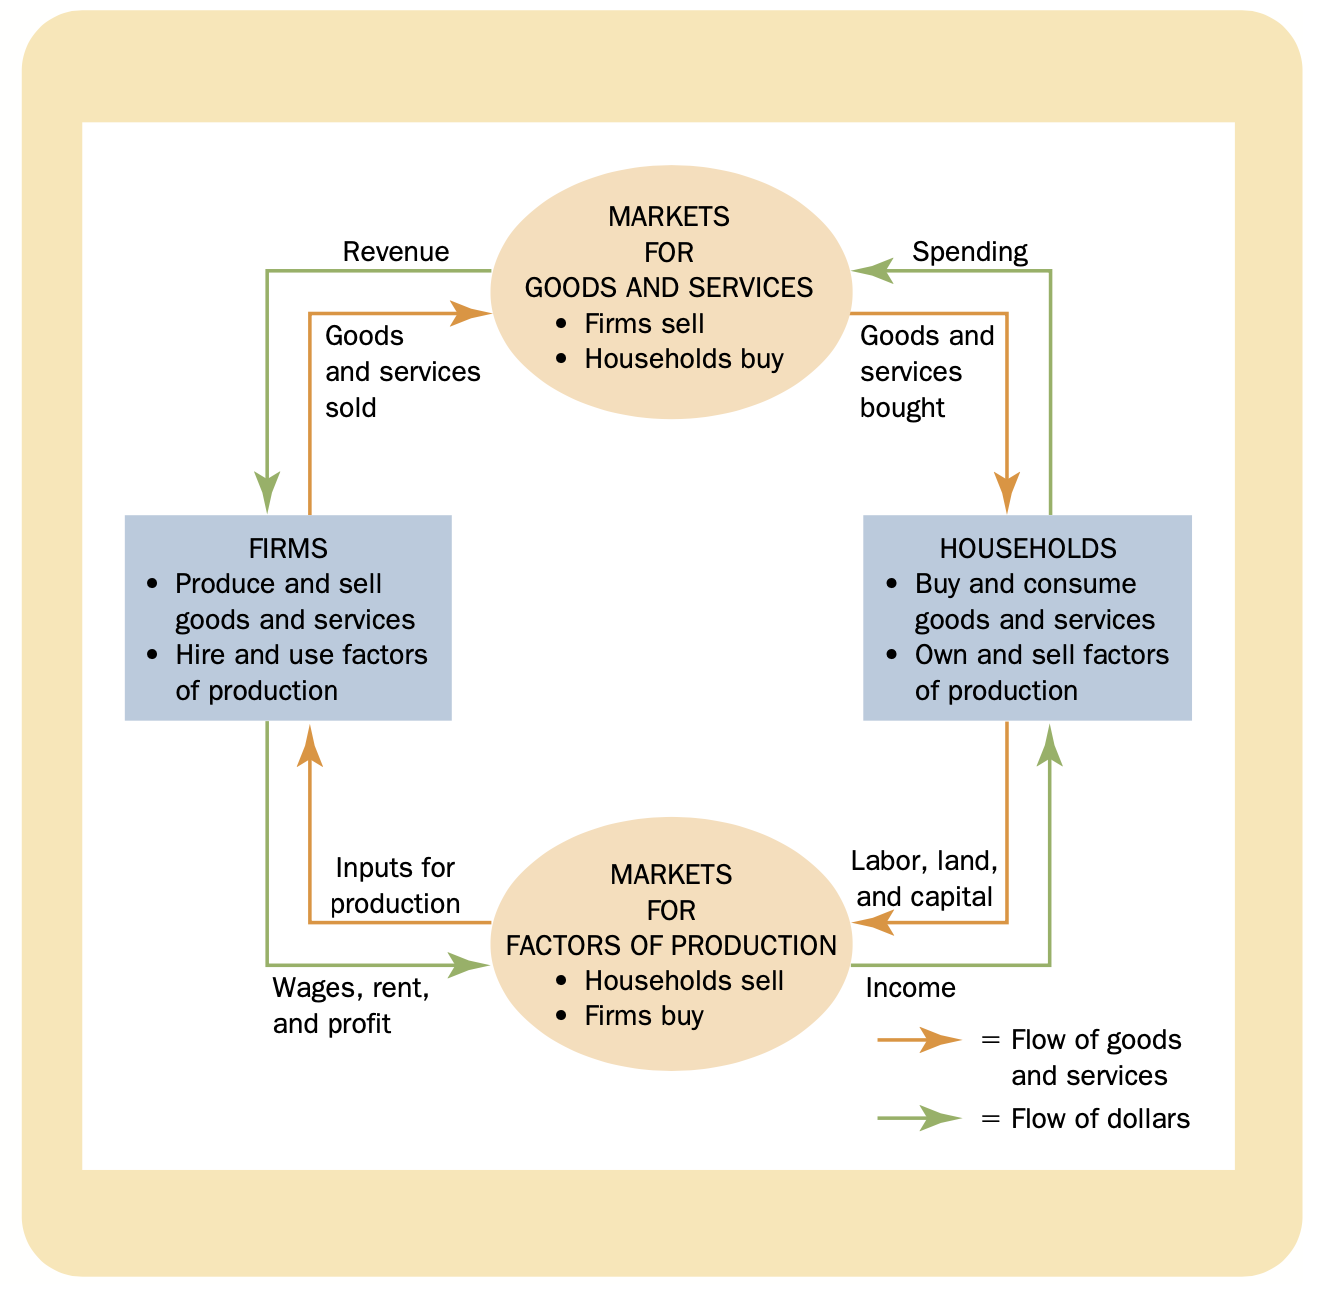
\includegraphics[width=\textwidth]{pics/circular-flow}
  \caption{循环流量图}
  \label{fig:circular-flow}
\end{figure}

在这个模型中,经济简化为只有两类决策者--企业家和家庭--组成。
企业用劳动、土地和资本(建筑物和机器)这些投入品来生产物品和服务。
这些投入品被称为生产要素。
家庭则拥有生产要素并消费企业家的所有物品与服务。


家庭和企业在两类时常上相互交易。
在物品和服务市场上,家庭是买者,而企业是卖者。
在生产要素市场上,家庭是卖者,而企业家是买者。
循环流量图提供了一种把家庭与企业之间发生的所有经济交易组织在一起的简单方法。


\subsection{生产可能性边界}

\begin{figure}[!ht]
  \centering
  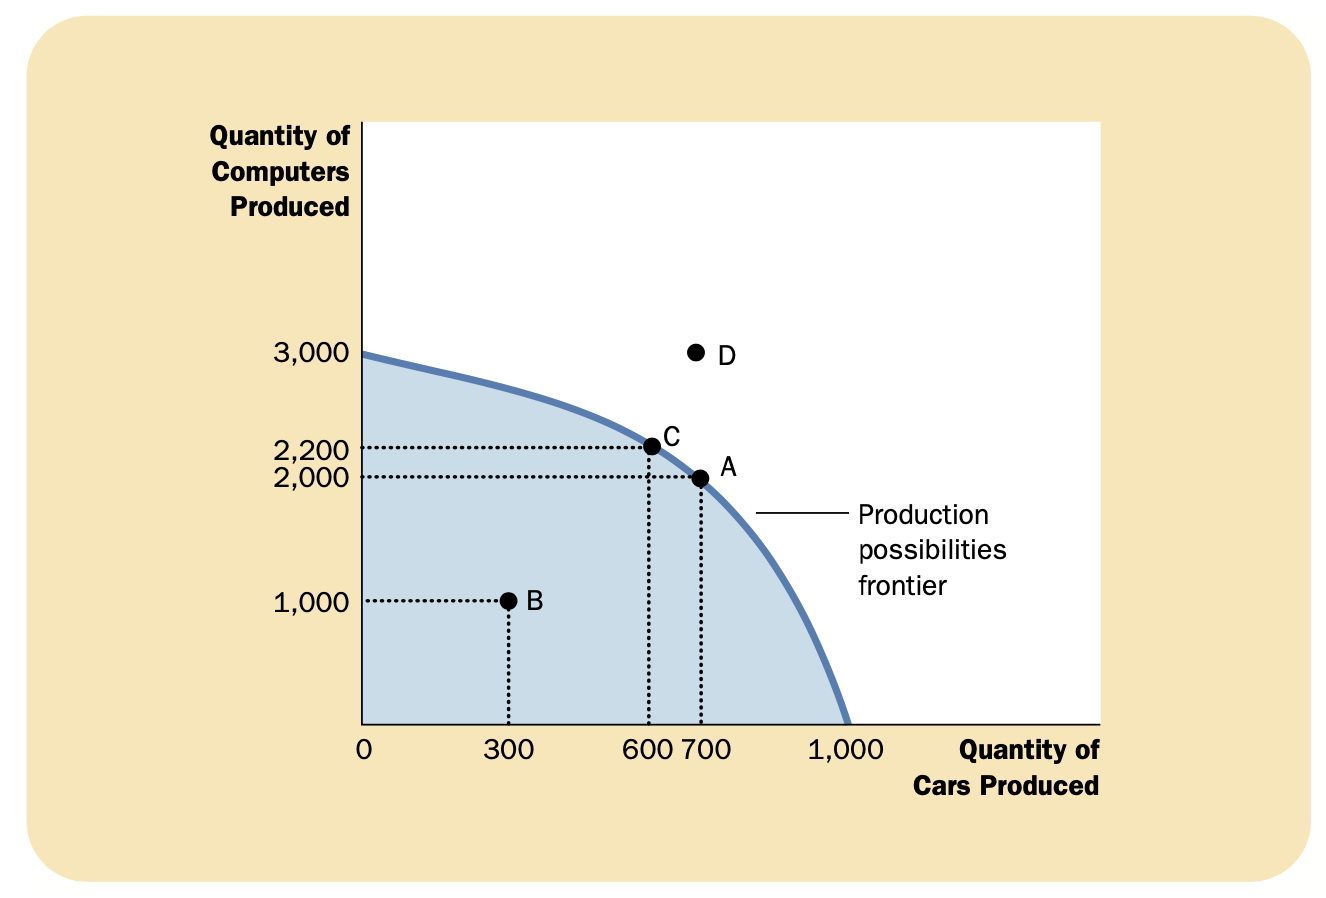
\includegraphics[width=\textwidth]{pics/the-production-possibilities-frontier}
  \caption{生产可能性边界}
  \label{fig:the-production-possibilities-frontier}
\end{figure}


虽然现实经济成千上万种物品和服务,但我们可以设想一个只生产两种物品--汽车和电脑--的经济。
生产可能性边界是一个图形,
它表明在生产要素和生产技术既定时,
一个经济所能生产的产品--在这个例子中是汽车和电脑--的数量的各种组合。


由于资源是稀缺的,因此并不是每一个想象的结果都是可行等等。
例如无法生产出D点所表示的汽车和电脑量。


如果一个经济从它可以获得的稀缺资源中获得它得到的全部东西,
就称这种结果是\emph{有效率}的。
生产可能性边界上(而不是这条线之内)的点代表了有效率的生产水平。

生产可能性边界表明在某一特定时期内生产不同物品之间的权衡取舍,
但随着时间的推移,
这种权衡取舍可以改变。

\begin{figure}[!ht]
  \centering
  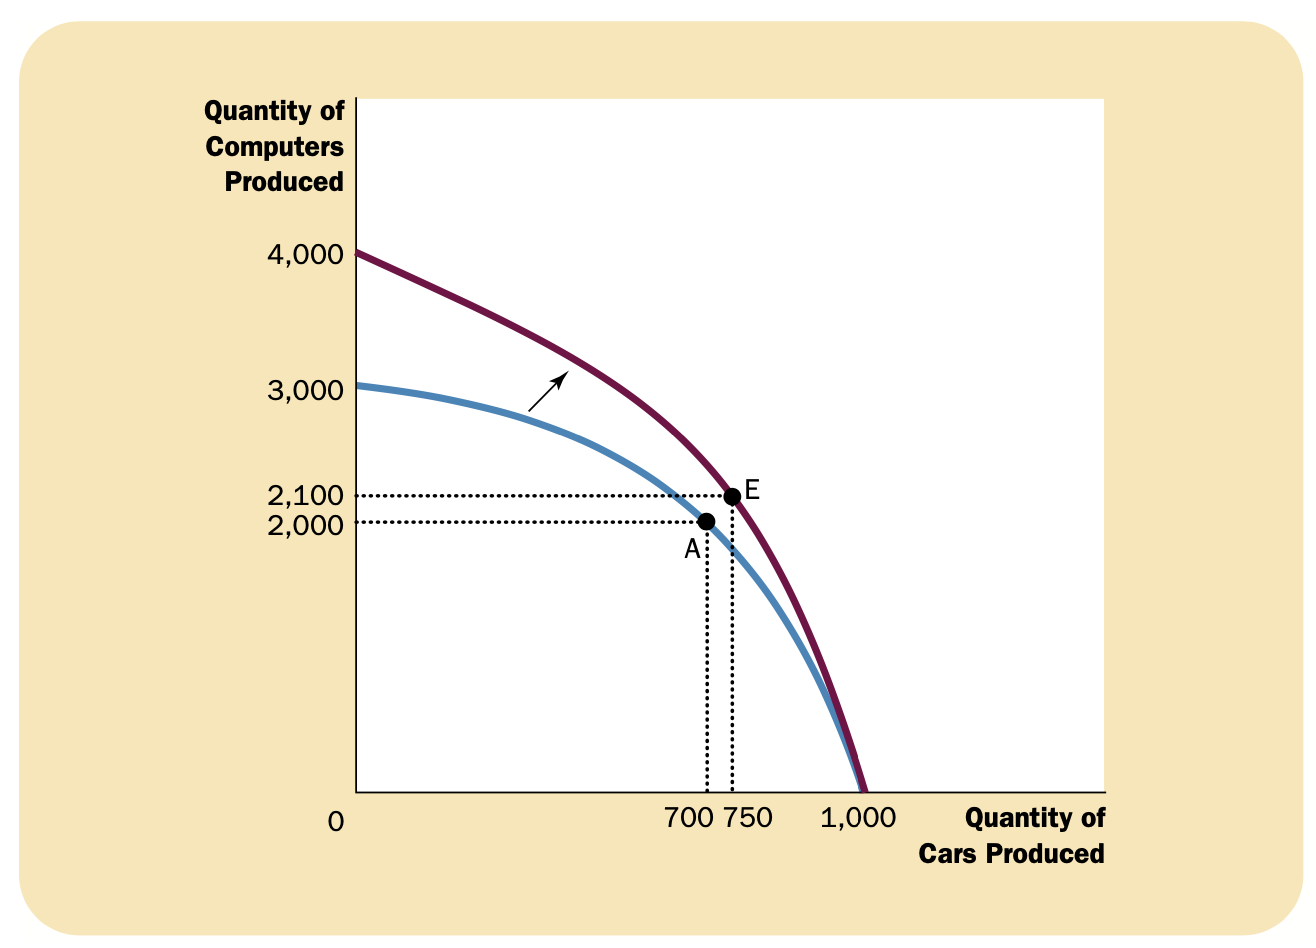
\includegraphics[width=\textwidth]{pics/a-shift-in-the-production-possibilities-frontier}
  \caption{生产可能性边界的移动}
  \label{fig:a-shift-in-the-production-possibilities-frontier}
\end{figure}


图\ref{fig:a-shift-in-the-production-possibilities-frontier}说明当经济增长时会发生的情况(例如生产电脑的技术水平的提高)。



生产可能性边界简化了复杂的经济,
以便强调一些基本但极为重要的思想:
稀缺性,效率,权衡取舍,机会成本和机会增长。




\subsection{微观经济学和宏观经济学}

经济学家在各种不同的层次上进行研究。
传统上,经济学被划分为两个大的分领域。
微观经济学研究家庭和企业如何做出决策,
以及他们如何在特定市场上相互交易。
宏观经济学研究整体经济现象。


\section{作为政策顾问的经济学家}

当经济学家试图去解释世界时,他们时科学家;
当经济学家试图去改善世界时,他们时政策顾问。



\subsection{实证分析与规范分析}

由于科学家和政策顾问有不同的目标,
所以他们也以不同的方式使用语言。


例如,假设两个人在讨论最低工资法。
\begin{verbatim}
张三:最低工资法引起失业。
李四:政府应该提高最低工资。
\end{verbatim}

张三和李四想做的事情时不同的。
张三的说法像一个科学家,他做出了一种关于世界如何运行的表述。
李四的说法像一个政策顾问,他做出了他想如何改变世界的表述。


一般来说,关于世界的表述有两种类型。
第一种类型的表述是实证的。
实证表述是描述性的,它们做出关于世界\emph{是}什么样子的表述。
第二种类型的表述是规范性的。
规范表述是规定性的,它做出关于世界\emph{应该是}什么样子的表述。


经济学的许多内容是实证的:它仅仅在努力解释世界如何运作。
但那些运行经济学的经济学家们通常有规范的目的:他们想知道如何改善经济。


\begin{verbatim}
   经济学家和政治哲学家的思想,无论正确与否,实际上都要比一般
所想象的更有力量。事实上,这个世界就是由他们统治的。那些自认为
能够免于受经济学家影响的实干家往往是某些已故经济学家的俘虏。那
些当权狂人信奉的其实也不过是若干年前某些末流文人狂妄思想的零碎
而已。                    ---- John Maynard Keynes
\end{verbatim}


\section{经济学家意见分歧的原因}

“如果让所有的经济学家围坐在一起,他们不会达成任何一个共识。”
George Bernard Shaw对经济学家的嘲讽从这句话中可见一斑。


为什么经济学家往往给决策者提供相互矛盾的建议呢?
这里有两个基本原因:
\begin{itemize}
\item 经济学家可能对世界如何运行的不同实证理论的正确性看法不一致。
\item 经济学家可能有不同的价值观,因此对政策应该努力实现的目标有不同的规范观点。
\end{itemize}


\subsection{感觉与现实}


由于科学判断的差别和价值观的不同,
经济学家之间有一些分歧是不可避免的,
但不应该夸大这种分歧。
经济学家之间的共识程度远远超出了人们有时认为的那样。


\begin{verbatim}
对专业的经济学家来说,网络游戏可能是下一个前沿。
\end{verbatim}
网游里的数据相当丰富。
而且,在网游中进行全面经济实验要容易的多。



\begin{verbatim}
经济学研究似乎并不需要任何极高的特殊天赋。与更高深的哲学或
纯科学相比,经济学难道不是...一门及其容易的学科吗?它是一门
容易的学科,但这个学科中很少有人能出类拔萃!对这个悖论的解释
也许在与杰出的经济学家应该具有罕见的各种天赋的组合。在某种
程度上,他们应该是数学家、历史学家、政治家和哲学家。他必须
了解符号符号并用文字将其表达出来。他必须根据一般性来深入思考
特殊性,并在思绪奔放的同时触及抽象与具体。他必须根据过去、
着眼现在而研究未来。他必须考虑到人性和人的制度的每一部分。
他必须同时保持坚定而客观的情绪,要像艺术家一样超然而不流俗,
但有时又要像政治家一样脚踏实地。
\end{verbatim}


\subsection{原因与结果}

当你看到一幅图被用于支持一种关于原因和结果的观点时,
应当问一下,
有没有一种被忽略的变量的变动能解释你观察到的结果,
这一点时很重要的。



% 
\chapter{相互依存性与贸易的好处}

你每天都在想用许多素不相识的人向你提供的物品与服务。
这种相互依存之所以成为可能,
是因为人们互相交易。
那些为你提供物品和服务的人并不是出于仁慈而这样做的。
相反,人们向你和其他消费者提供他们生产的物品与服务,
是因为他们也得到了某种回报。




\section{比较优势:专业化的动力}

\subsection{绝对优势}


当比较一个人、一个企业或者一个国家与另一个人、另一个企业或另一个国家的生产率时,
经济学家用\keyword{绝对优势}这个术语。
如果生产者生产一种物品所需要的投入较少,
就可以说该生产者在生产这种物品上有绝对优势。


\subsection{机会成本和比较优势}



在描述两个生产者的机会成本时,经济学家用\keyword{比较优势}这个术语。
如果一个生产者在生产X物品时放弃了较少的其他产品,
即生产X物品的机会成本较小,
我们就可以说,他在生产该物品上具有比较优势。


今天一个人有可能在两种物品的生产上都有绝对优势,
但一个人却不可能在两种物品的生产上都具有比较优势。
因为一种物品的机会成本是另一种物品机会成本的倒数,
(除非两个人有相同的机会成本)。
比较优势反应了相对的机会成本。


\subsection{比较优势与贸易}

专业化和贸易的好处不是基于绝对优势,
而是基于比较优势。
当每个人专门生产自己比较优势的物品时,
经济的总产量就增加了,
经济蛋糕的变大可用于改善每个人的状况。
人们通过以低于自己生产某种物品的机会成本的价格得到该物品而从贸易中获益。



贸易可以使社会上每个人都获益,
因为它使人们可以专门从事他们具有比较优势的互动。


\subsection{贸易的价格}

对从贸易中获益的双方而言,
他们进行贸易的价格在两种机会成本之间。


\subsection{比较优势的应用}


一位经济学家认为,你不应该仅仅因为你比你的配偶更擅长洗碗,就总是负责洗碗。
(比较优势)



% 
\chapter{供给与需求的市场力量}

\keyword{供给}与\keyword{需求}是经济学家最经常使用的两个词。
供给与需求是使市场经济运行的力量。
它们决定了每种物品的产量及其出售的价格。
如果你想知道一件事件或政策如何影响经济,
你就应该先考虑它将如何影响供给和需求。


\section{市场与竞争}

供给与需求是指人们在竞争市场上互相交易时的行为。

\subsection{什么是市场}

市场是由某种物品或服务的买者与卖者组成的一个群体。
买者作为一个群体决定了一种产品的需求,
而卖者作为一个群体决定了一种产品的供给。


\subsection{什么是竞争}

经济学家用\keyword{竞争市场}来描述有许多买者与卖者并且每一个人对市场价格的影响都微乎其微的市场。


\keyword{完全竞争}的市场必须具备两个特征:
\begin{itemize}
\item 可供销售的物品是完全相同的。
\item 买者和卖者人数众多,以至于没有任何一个买者或卖者可以影响市场价格。
\end{itemize}
由于完全竞争市场上的买者与卖者都必须接受市场决定的价格,
所以他们被成为\keyword{价格接受者}。


并不是所有物品与服务都在完全竞争市场上出售。
一些市场只有一个卖者,
而且这个卖者决定价格,
这样的卖者被称为\keyword{垄断者}。


\section{需求}

\subsection{需求曲线:价格和需求量之间的关系}

一种物品的\keyword{需求量}是买者愿意并且能够购买的该种物品的数量。

需求定理:在其他条件不变时,一种物品的价格上升,对该物品的需求量减少;
一种物品的价格下降,对该物品的需求量增加。

\begin{figure}[!ht]
  \centering
  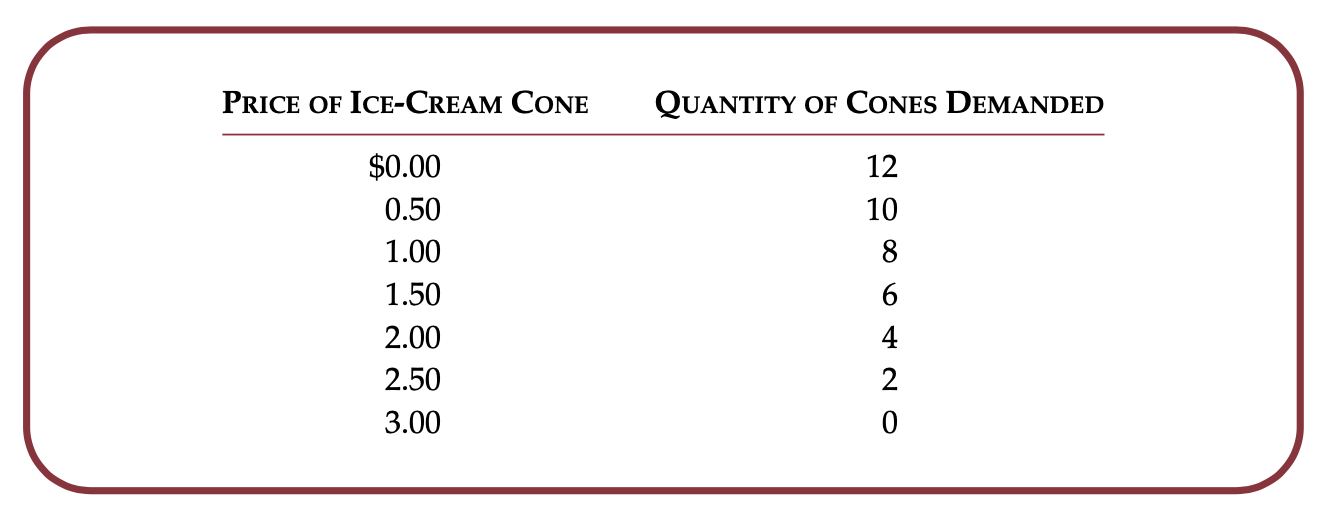
\includegraphics[width=\textwidth]{pics/demand-schedule}
  \caption{需求表}
  \label{fig:demand-schedule}
\end{figure}

表\ref{fig:demand-schedule}是一个需求表,
它表明在影响消费者想购买的数量的其他因素都保持不变的情况下,
一种物品的价格与其需求量之间的关系。

\begin{figure}[!ht]
  \centering
  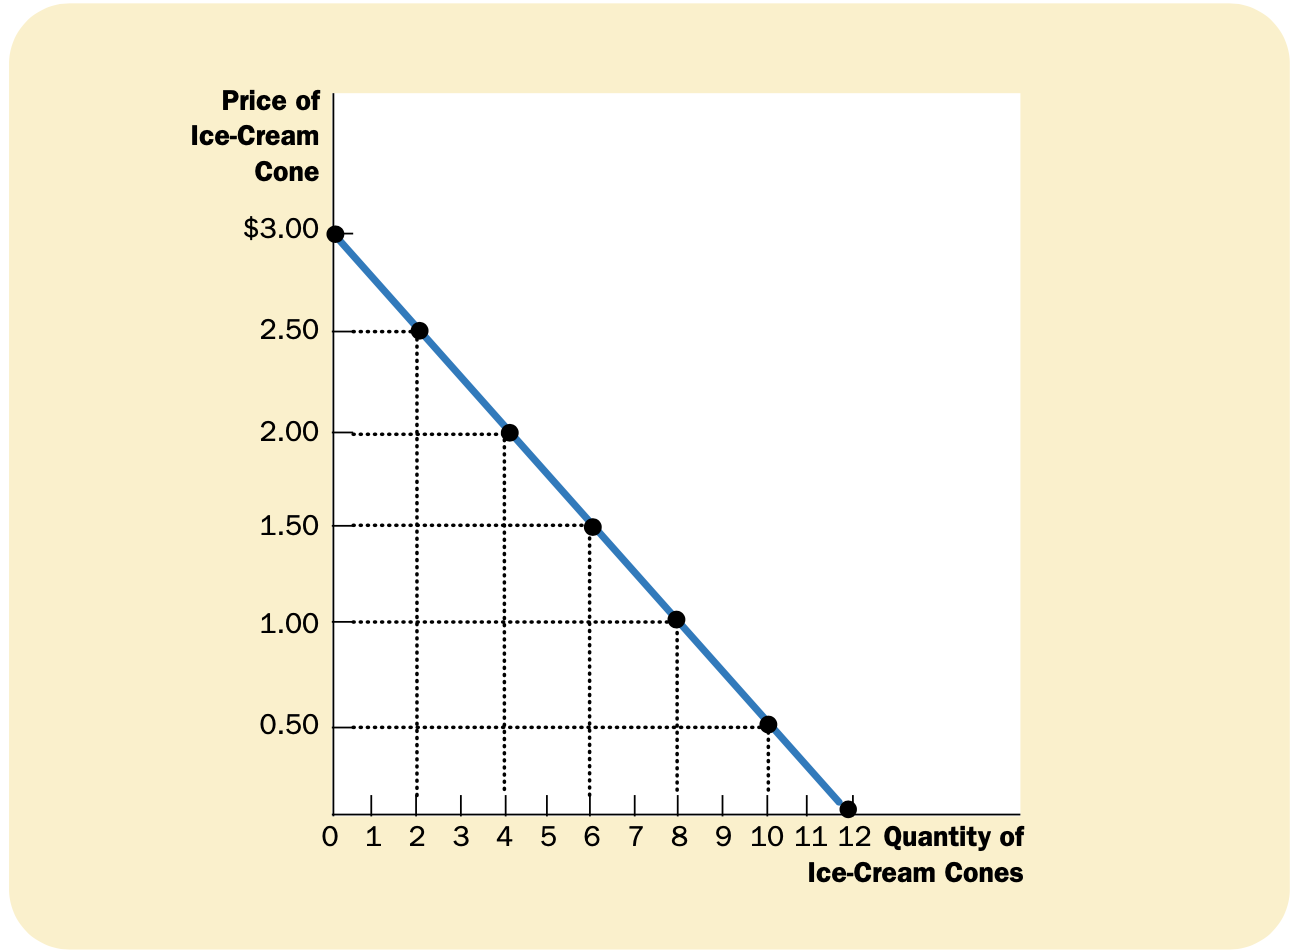
\includegraphics[width=\textwidth]{pics/demand-curve}
  \caption{需求曲线}
  \label{fig:demand-curve}
\end{figure}

图\ref{fig:demand-curve}表示需求曲线,
它把价格和需求量联系在一起。


\subsection{市场需求与个人需求}

市场需求是所有个人对某种特定物品或服务的需求的总和。


\subsection{需求曲线的移动}

由于市场需求曲线假设其他条件不变,
但随着时间的推移,
该曲线不一定是稳定的,
如果某个因素改变了任何一种既定价格水平的需求量,
需求曲线就会移动。


有许多变量会是需求曲线移动。
以下是一些最重要的变量:
\begin{itemize}
\item 收入
\item 相关物品的价格
\item 爱好
\item 预期
\item 买者的数量
\end{itemize}

当收入减少时,如果一种物品的需求量减少,这种物品就被称为\keyword{正常物品}。
当收入减少时,如果一种物品的需求量增加,这种物品就被称为\keyword{低档物品}。
当一种物品价格下降一起对另一种物品的需求量减少时,这种物品就被称为\keyword{替代品}。
当一种物品价格下降一起对另一种物品的需求量增加时,这种物品就被称为\keyword{互补品}。


\section{供给}

\subsection{供给曲线:价格与供给量之间的关系}

一种物品或者服务的\keyword{供给量}是卖者愿意并且能够出售的该种物品的数量。

供给定理:在其他条件不变时,一种物品价格上升,该物品供给增加;
一种物品价格下降,该物品供给减少。

供给表:在影响某种物品的生产者想出售数量的其他因素都保持不变的情况下,
该物品的价格和供给量之间的关系。

供给曲线:把价格和供给量联系在一起的曲线。



\subsection{市场供给与个人供给}

市场供给是所有卖者供给的总和。


\subsection{供给曲线的移动}


由于市场供给曲线假设其他条件不变,
当这些因素中的一个因素变动时,
该曲线将会发生移动。



有许多变量会使供给曲线移动,
以下是一些最重要的变量:
\begin{itemize}
\item 投入品价格
\item 技术
\item 预期
\item 卖者的数量
\end{itemize}


\section{供给与需求的结合}

\subsection{均衡}

\begin{figure}[!ht]
  \centering
  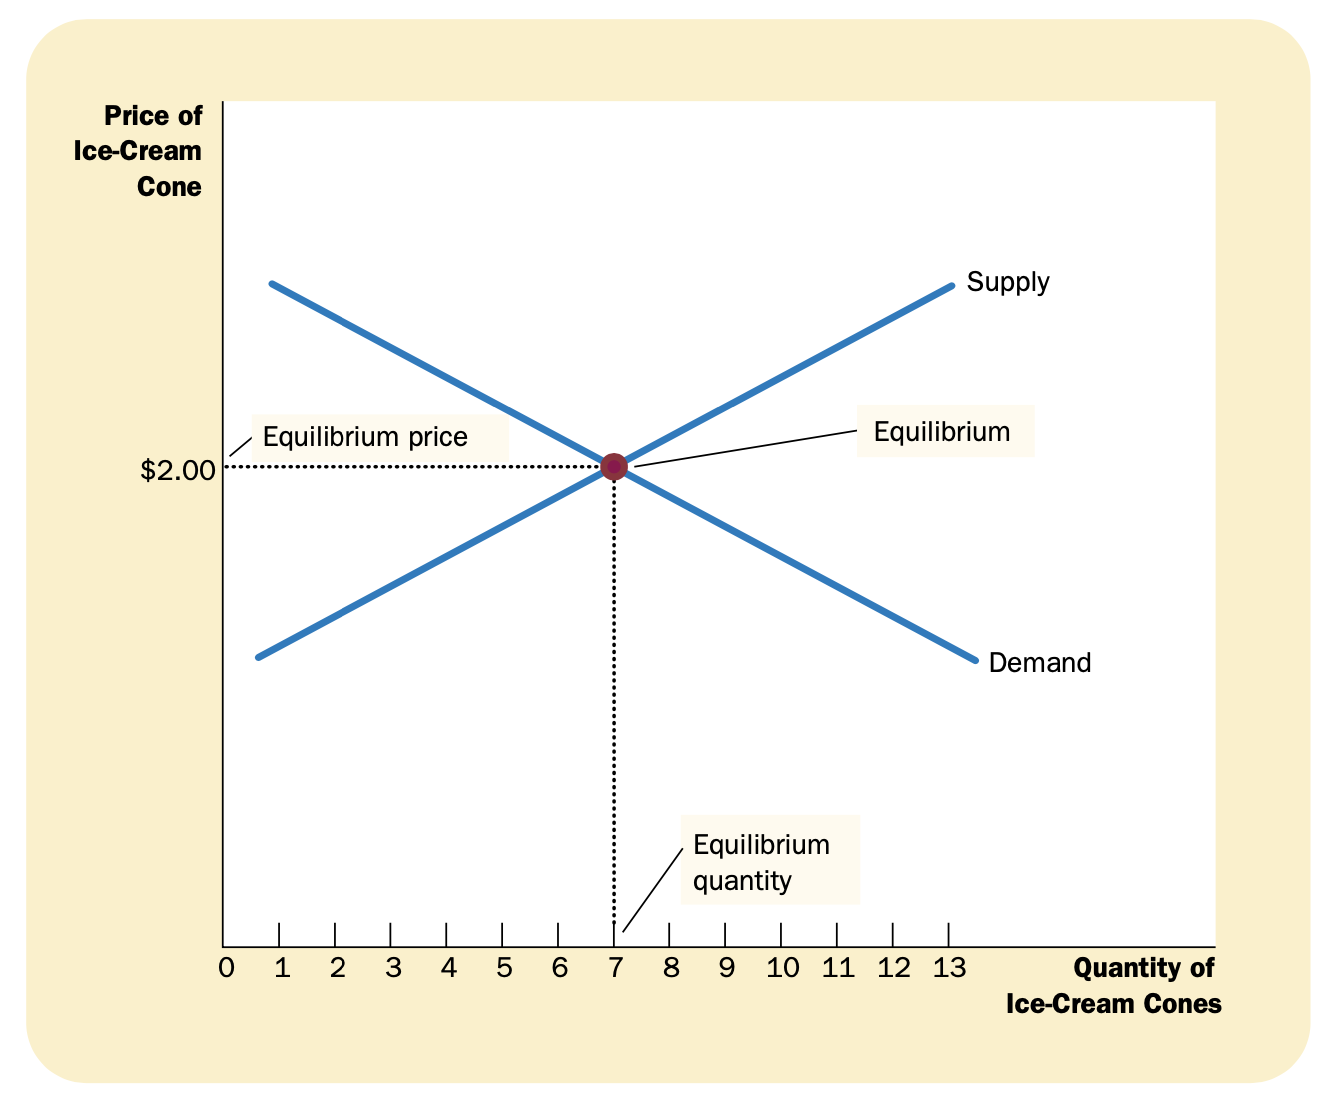
\includegraphics[width=\textwidth]{pics/equilibrium-of-supply-and-demand}
  \caption{供给与需求的均衡}
  \label{fig:equilibrium-of-supply-and-demand}
\end{figure}

图\ref{fig:equilibrium-of-supply-and-demand}同时给出了市场供给曲线和市场需求曲线。
供给曲线和需求曲线相较于一点,这一点被称为市场的\keyword{均衡}。
这两条曲线相交时的价格被称为\keyword{均衡价格},
而相交时的数量被称为\keyword{均衡数量}。


供求定理:任何一种物品的价格都会自发调整,使该物品的供给与需求达到平衡。


\subsection{分析均衡变动的三个步骤}

供给和需求共同决定了市场均衡,
市场均衡又决定了物品价格,
以及买者所购买和卖者所生产的该物品数量。
均衡价格和均衡数量取决于供给曲线和需求曲线的位置。
当某些事件使一种一条曲线移动时,
市场上的均衡就改变了,
从而将在买者和卖者之间产生新的均衡价格和均衡数量。



当分析某个事件如何影响一个市场上的均衡的时候,
我们按三个步骤进行:
\begin{enumerate}
\item 确定该事件是使供给曲线还是需求曲线移动,还是使两条曲线都移动。
\item 确定曲线是向右移动,还是向左移动。
\item 用供求图来比较原来的均衡和新均衡,以说明这种移动如何影响均衡价格和均衡数量。
\end{enumerate}


供给曲线的移动被称为“供给变动”,
而需求曲线的移动被称为“需求变动”。
沿着一条固定供给曲线的变动称为“供给量的变动”,
而沿着一条固定需求曲线的变动称为“需求量的变动”。


\begin{tcolorbox}
  哄抬物价是变相抢劫吗?

  道德掺合进经济学里对法律肯定是有害的。
  只有在需求的物品出现短缺的情况下,哄抬物价才会出现。
  如果没有短缺,正常的市场过程会阻止物价突然上升。

  在极端需求情况下允许价格上涨限制了过度消费。
  人们会更仔细地考虑他们的购买。
  结果在极端的情况下会又更多的顾客买得到物品。
  市场过程的结果实际上比反哄抬物价更能实现较为平等的分配。

  商人实际上并没有从灾难中获利,
  商人是通过对物价的管理来获利的,
  这种对自己物价的管理实际上扩大了商品的分配范围,
  并限制了囤积居奇,
  从而产生了有益的社会效应。
  简言之,他们是由于提供了重要的公共服务而正当地获得了回报。
\end{tcolorbox}


\section{价格如何配置资源}

供给和需求共同决定了经济中许多不同物品与服务的价格,
而价格又是引导资源配置的信号。
在市场经济中,价格是配置稀缺资源的机制。







% 
\chapter{弹性及其应用}

弹性衡量买者与卖者对市场条件变化的反应程度。

\section{需求弹性}

\subsection{需求价格弹性及其决定因素}

\keyword{需求价格弹性}衡量需求量对价格变动的反应程度。
如果一种物品的需求量对价格变动的反应很大,
就说明这种物品的需求量是\keyword{富有弹性}的。
如果一种物品的需求量对价格变动的反应很小,
就说明这种物品的需求是\keyword{缺乏弹性}的。


由于需求反映了形成消费者偏好的许多经济、社会与心理因素,
所有没有一个决定需求曲线弹性的简单而普遍的规律。
但根据经验,我们可以总结出某些决定需求价格弹性的经验法则。

\begin{description}
\item[相似替代品的可获得性] 有相似替代品的物品的需求往往较富有弹性。
\item[必需品与奢侈品] 必需品的需求往往缺乏弹性,而奢侈品的需求往往富有弹性。
\item[市场的定义] 任何一个市场上的需求弹性都取决于我们如何划定市场的边界。狭窄定义的市场的需求弹性往往大于宽泛定义的市场的需求弹性,因为狭窄定义的市场长的物品更容易找到相近的替代品。
\item[时间范围] 物品的需求往往在长期内更富有弹性。
\end{description}



\subsection{需求价格弹性的计算}

\begin{equation}
  \text{需求价格弹性} = \frac{\text{需求量变动百分比}}{\text{价格变动百分比}}
\end{equation}



\subsection{中点法:一个计算变动百分比和弹性的更好方法}

计算$(Q_1,P_1)$和$(Q_2,P_2)$两点间需求价格弹性的中点法可以用以下公式表示:
\begin{equation}
  \text{需求价格弹性} =
  \frac{
    \frac{Q_2-Q_1}{(Q_2+Q_1)/2}
  }{
    \frac{P_2-P_1}{(P_2+P_1)/2}
  }
\end{equation}


\subsection{各种需求曲线}

经济学家根据需求弹性对需求曲线进行分类。
当弹性大于1,需求是富有弹性的。
当弹性小于1,需求是缺乏弹性的。
当弹性等于1,需求是单位弹性的。



通过某一点的需求曲线越平坦,
需求价格弹性就越大;
通过某一点的需求曲线越陡峭,
需求价格弹性就越小。



\subsection{总收益与需求价格弹性}

\begin{figure}[!ht]
  \centering
  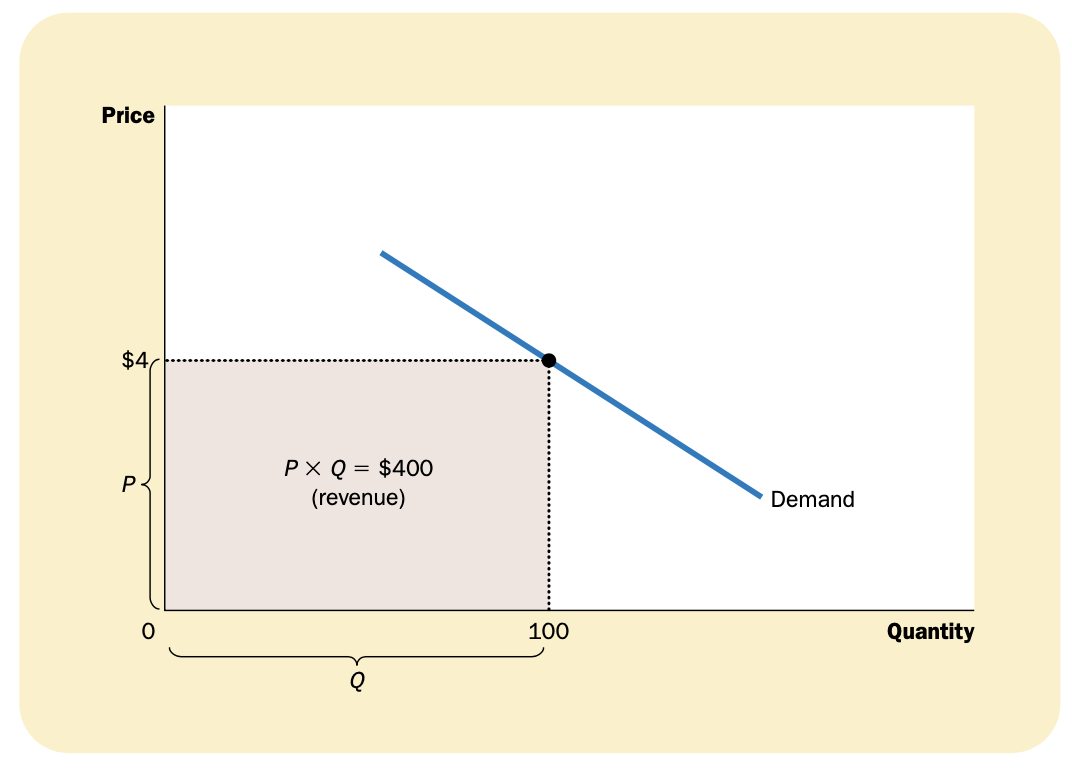
\includegraphics[width=\textwidth]{pics/total-revenue}
  \caption{总收益}
  \label{fig:total-revenue}
\end{figure}
如图\ref{fig:total-revenue}所示,
总收益是某种物品的买者支付从而卖者得到的量。
在任何一个市场上,总收益是$P\times Q$,
即一种物品的价格乘以该物品的销售量。


总收益如何沿着需求曲线变动呢?
答案取决与需求价格弹性。

\begin{figure}[!ht]
  \centering
  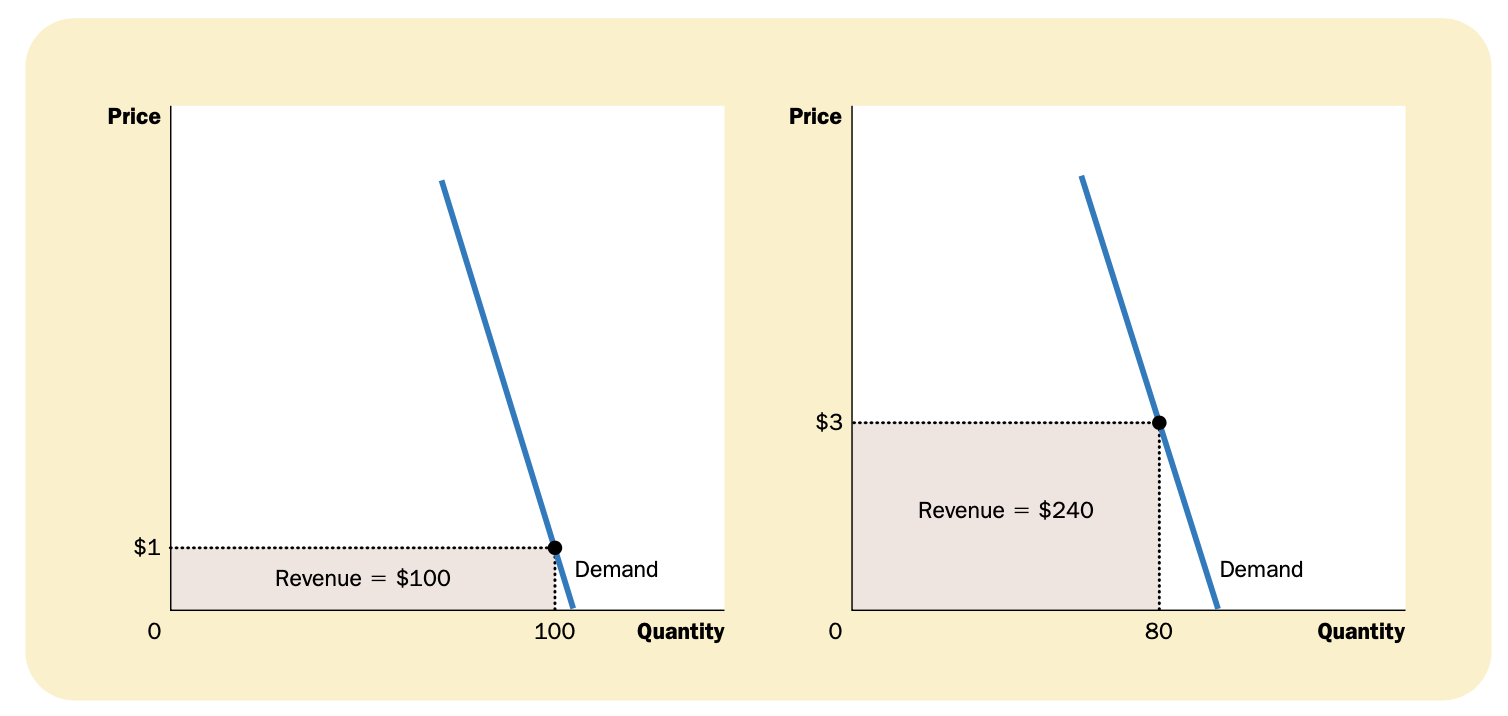
\includegraphics[width=\textwidth]{pics/inelastic-demand}  
  \caption{缺乏弹性}
  \label{fig:inelastic-demand}
\end{figure}

\begin{figure}[!ht]
  \centering
  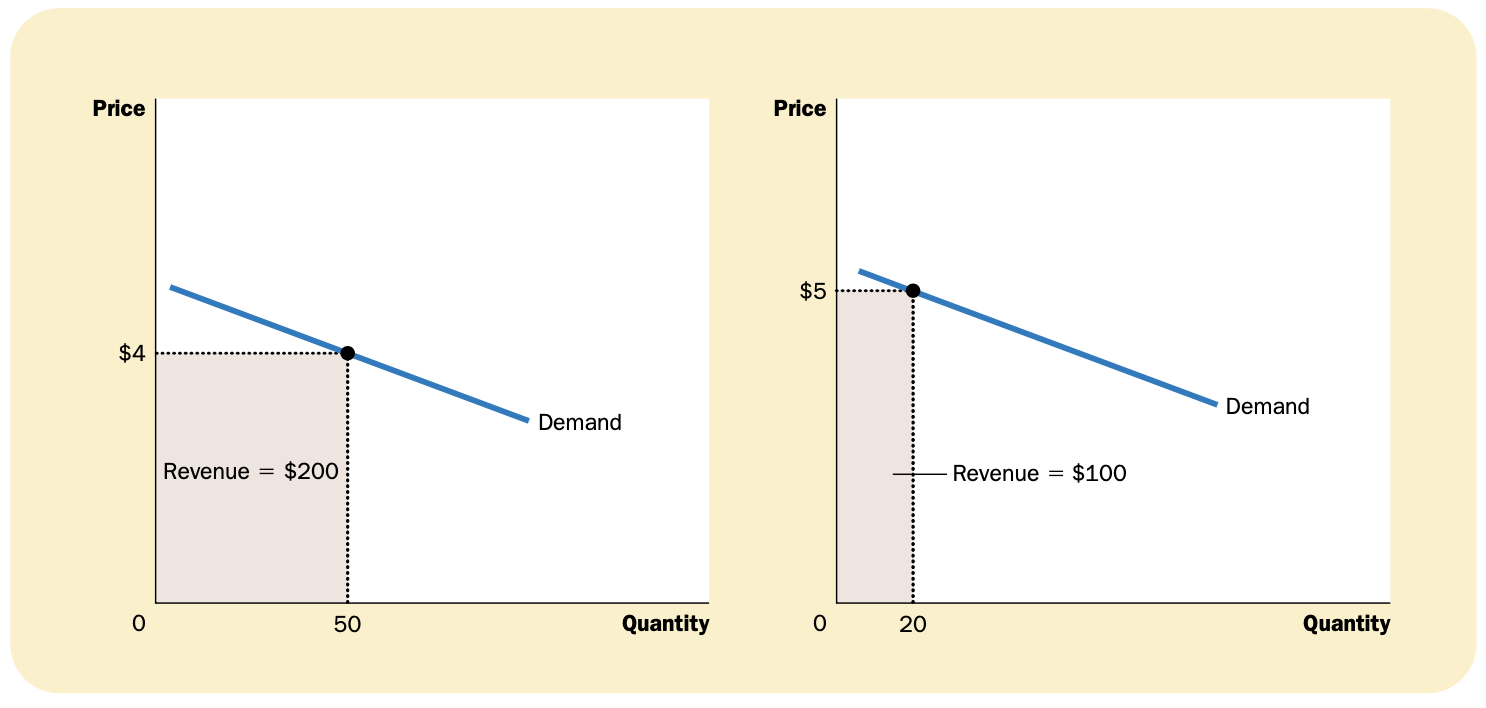
\includegraphics[width=\textwidth]{pics/elastic-demand}  
  \caption{富有弹性}
  \label{fig:elastic-demand}
\end{figure}


\begin{enumerate}
\item 当需求缺乏弹性(价格弹性小于1)时,价格和总收益同方向变动:如果价格上升,总收益增加。
\item 当需求缺乏弹性(价格弹性大于1)时,价格和总收益反方向变动:如果价格上升,总收益减少。
\item 如果需求是单位弹性的(价格弹性等于1)时,当价格变动时,总收益保持不变。
\end{enumerate}



\subsection{其他需求弹性}

\begin{equation}
  \text{需求收入弹性} = \frac{\text{需求量变动百分比}}{\text{收入变动百分比}}
\end{equation}

\begin{equation}
  \text{需求的交叉价格弹性} = \frac{\text{物品1的需求量变动百分比}}{\text{物品2的价格变动百分比}}
\end{equation}


\section{供给弹性}

\subsection{供给价格弹性及其决定因素}

\keyword{供给价格弹性}衡量供给量对价格变动的反应程度。
供给在长期中的弹性通常大于短期。


\subsection{供给价格弹性的计算}

\begin{equation}
  \text{供给价格弹性} = \frac{\text{供给量变动百分比}}{\text{价格变动百分比}}
\end{equation}


\subsection{各种供给曲线}

\begin{figure}[!ht]
  \centering
  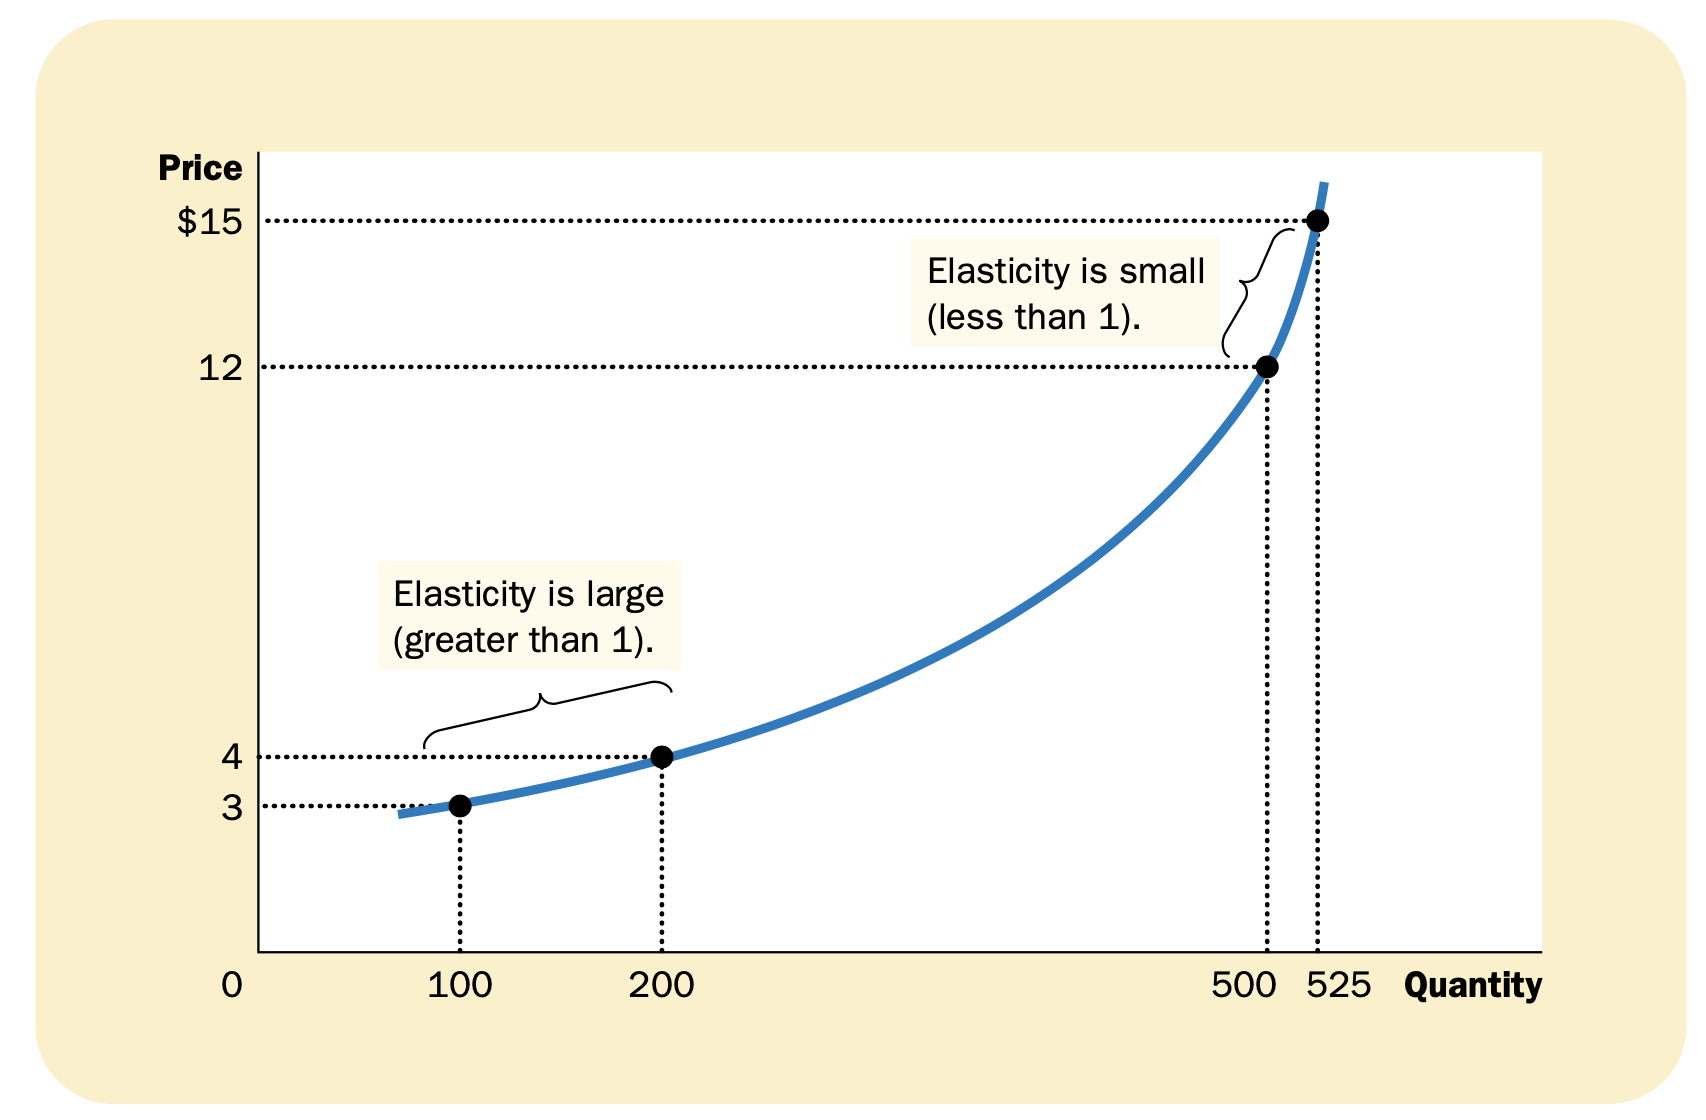
\includegraphics[width=\textwidth]{pics/supply-elastic-price}
  \caption{供给价格弹性的变动}
  \label{fig:supply-elastic-price}
\end{figure}



\section{供给、需求和弹性的应用}

\subsection{农业的好消息可能对农民来说是坏消息吗?}

\begin{figure}[!ht]
  \centering
  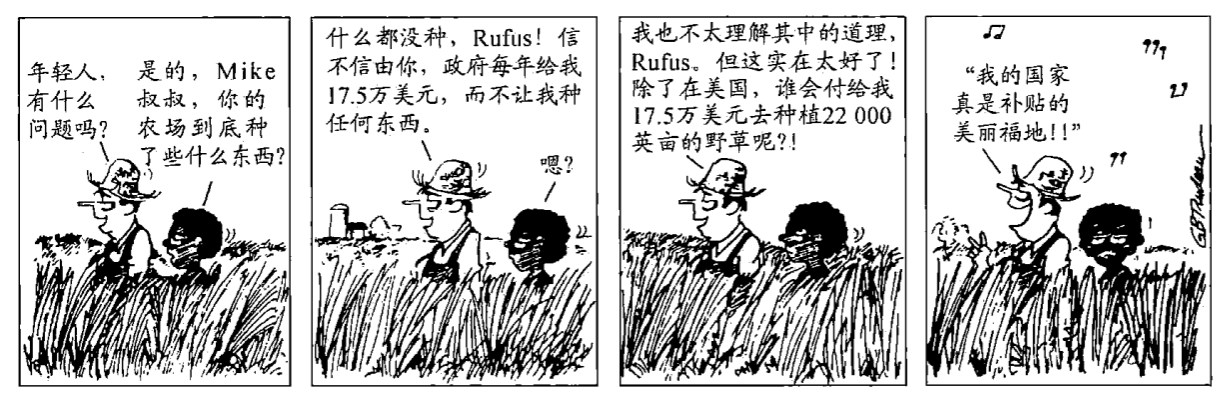
\includegraphics[width=\textwidth]{pics/farmer}
\end{figure}


对农民有力的不一定对整个社会也有利。
农业技术进步对农民而言可能是坏事,
因为它使农民逐渐变得不必要,
但对能以低价买到消费正而言可定是好事。
同样,旨在减少农产品供给的政策可以增加农民的收入,
但必然会以损害消费者的利益为代价。


\section{结论}

只要学会说“供给与需求”,甚至连一只鹦鹉都可能称为一个经济学家。
% 
\chapter{供给、需求与政府政策}

政府政策往往会产生一些其设计者没有想到或者没有预见到的影响。

\section{价格控制}

法定最高价格称为\keyword{价格上限}。
法定最低价格称为\keyword{价格下限}。


\subsection{价格上限如何影响市场结果}

价格上限高于均衡价格时,价格上限是\keyword{非限制性的}。
价格上限低于均衡价格时,价格上限是\keyword{限制性的}。

当政府对竞争市场实行限制性价格上限时,
就产生了物品的短缺,而且,
卖者必须在大量潜在的买者中配给稀缺物品。


\subsection{价格下限如何影响市场结果}
当政府对竞争市场实行限制价格下限时,
就产生了物品的过程,而且
同样会导致不合意的配给机制。


\subsection{对价格控制的评价}

在经济学家看来,
价格并不是某些偶然过程的结果。
他们认为,
价格是隐藏在供给曲线和需求曲线背后的千百万企业和消费者决策的结果。
价格有平衡供求从而协调经济活动的关键作用。
当决策者通过法令确定价格时,
他们就模糊了正常情况下指引社会资源配置的信号。


\section{税收}


税收归宿(tax incidence)这个术语是指税收负担如何在组成市场的不同人之间分配。


\subsection{向卖者征税如何影响市场}

\begin{figure}[!ht]
  \centering
  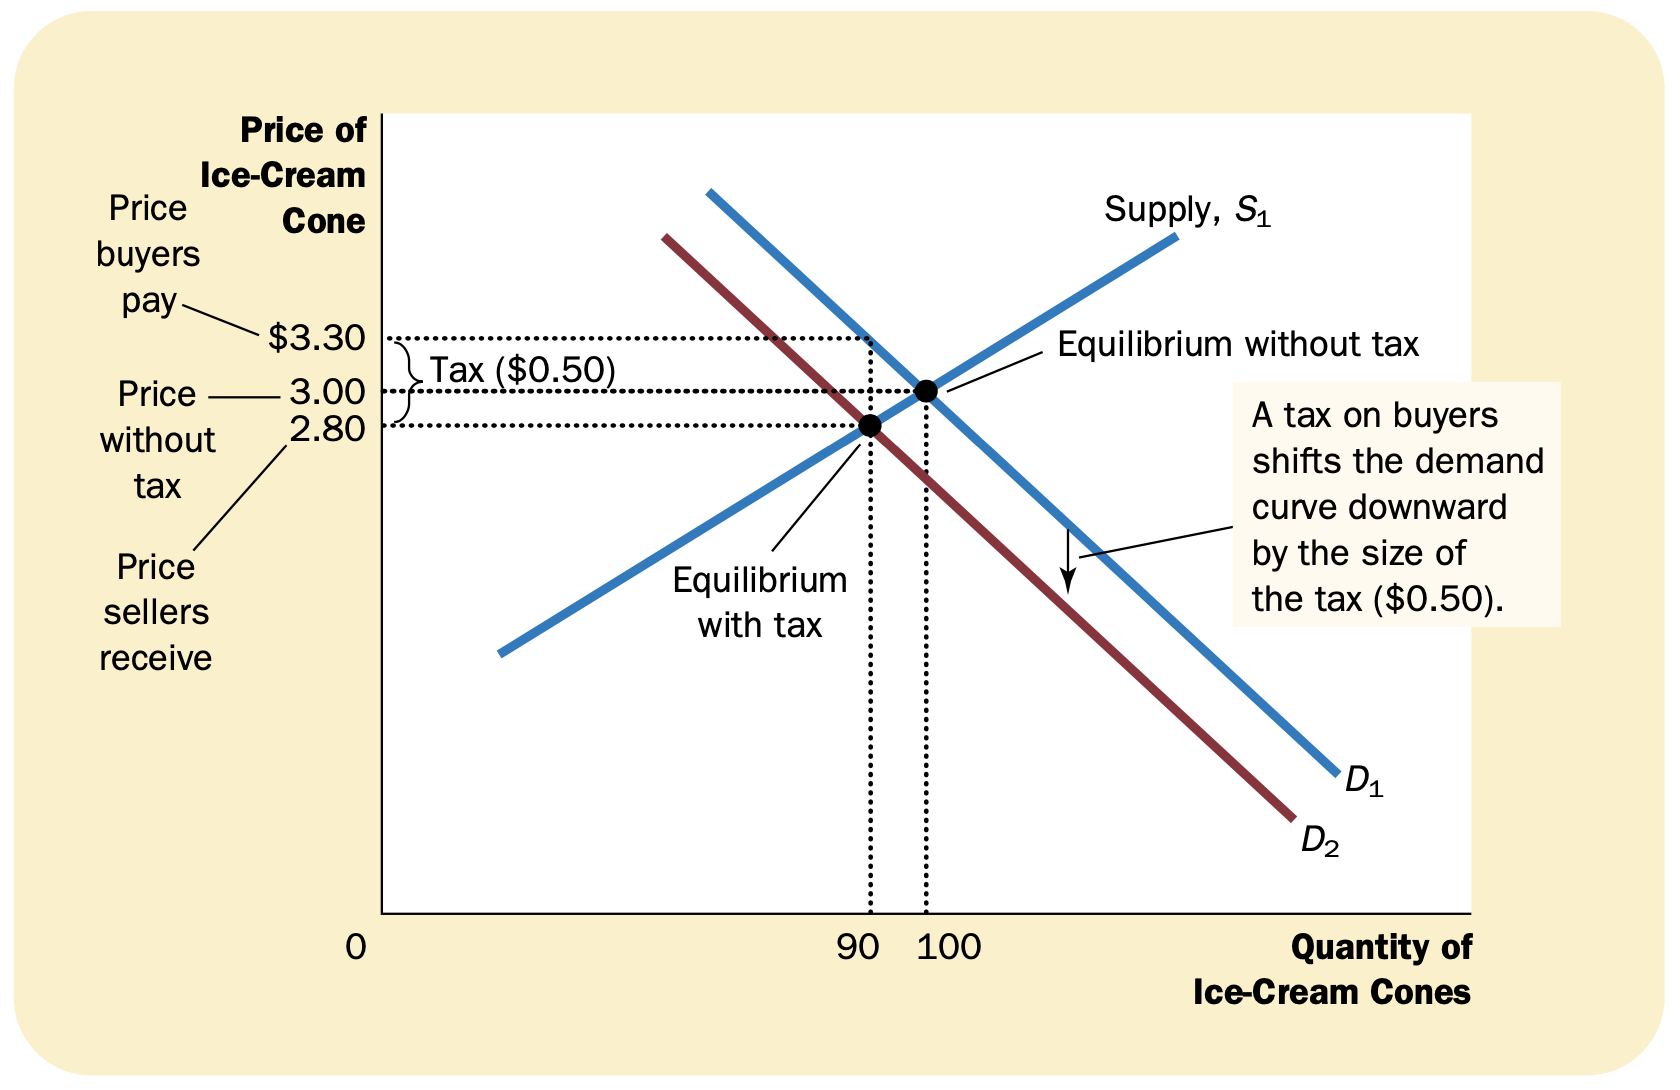
\includegraphics[width=\textwidth]{pics/tax1}
  \caption{向卖者征税}
  \label{fig:tax1}
\end{figure}


结论:
\begin{itemize}
\item 税收抑制了市场活动。当对一种物品征税时,该物品在新均衡时的销售量减少了。
\item 买者与买者分摊了税收负担。新均衡时,买者为该物品支付的更多了,而买者得到更少了。
\end{itemize}




\subsection{向买者征税如何影响市场}


\begin{figure}[!ht]
  \centering
  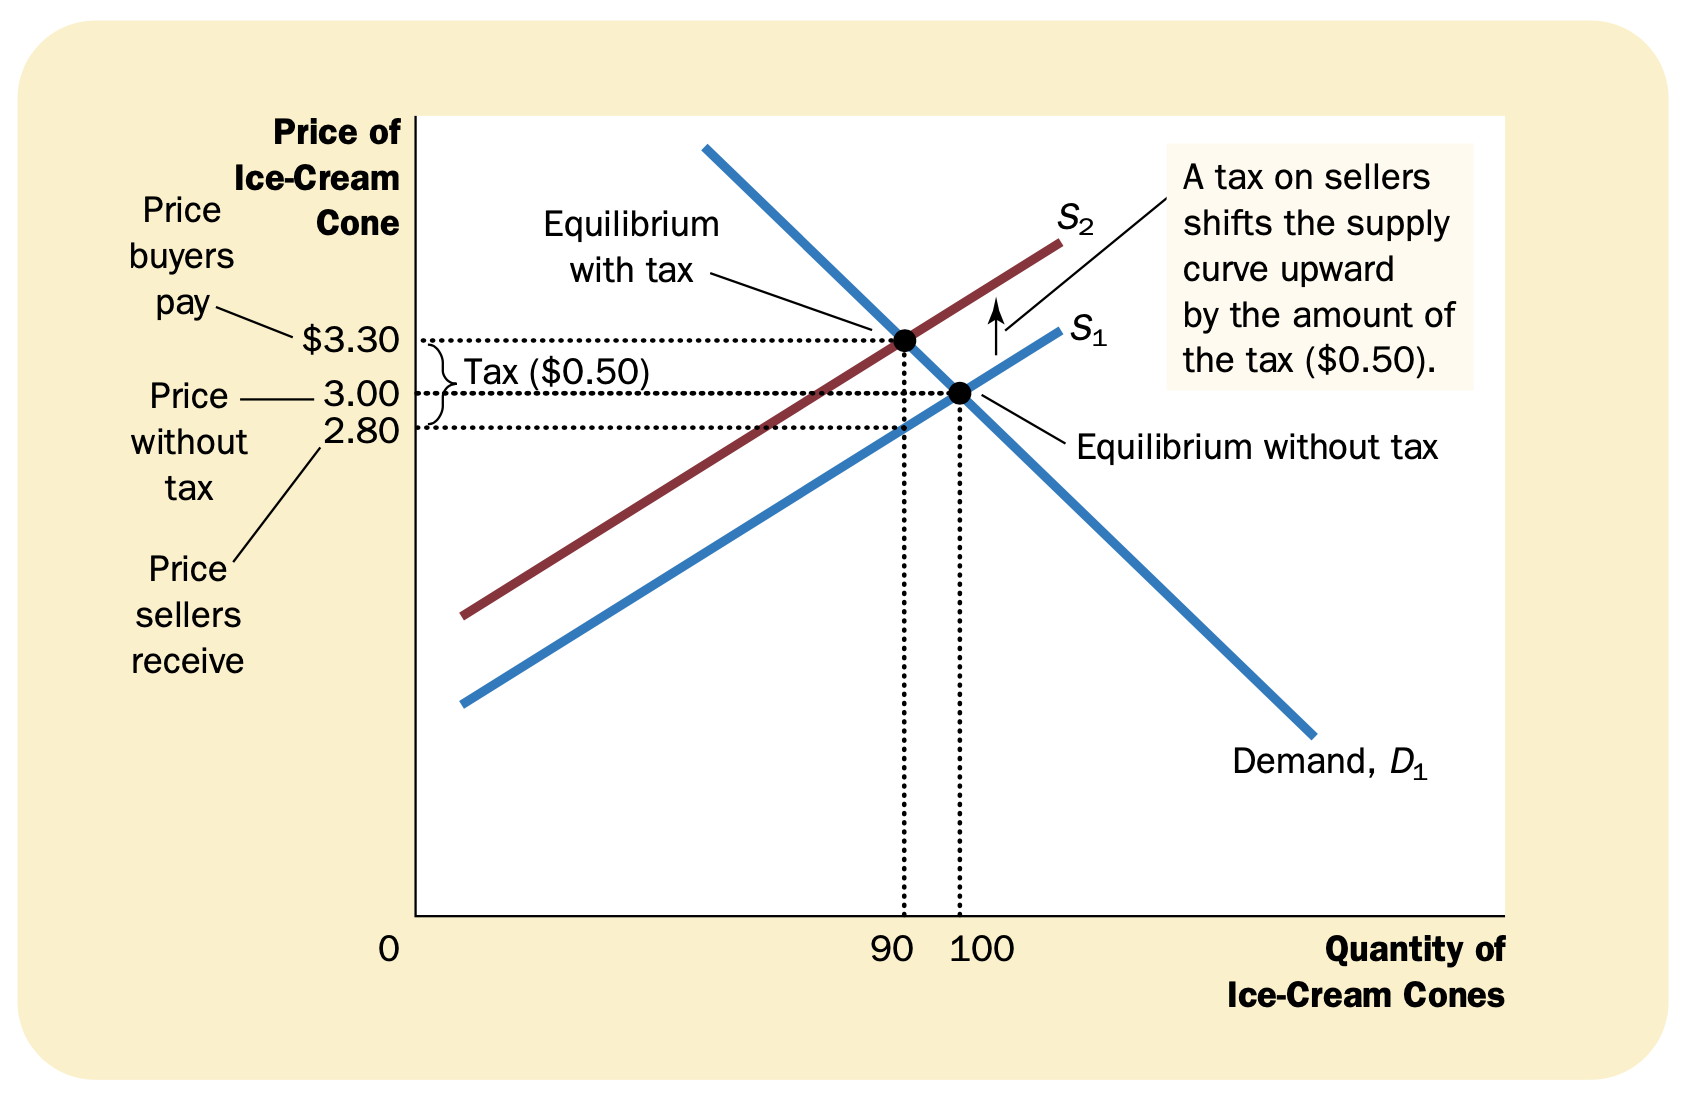
\includegraphics[width=\textwidth]{pics/tax2}
  \caption{向买者征税}
  \label{fig:tax2}
\end{figure}

结论:
对买者征税和对卖者征税是相同的。
对买者征税和对卖者征税的唯一区别是谁来把钱交给政府。




立法者可以决定税收是来自买者的口袋还是来自卖者的口袋,
但他们不能用立法规定税收的真正负担,
税收归宿取决于供给和需求的力量。




% 
\chapter{生产者、生产者与市场效率}

福利经济学(welfare economics):研究自研配置如何影响经济福利的一门学问。


\section{消费者剩余}

\subsection{支付意愿}

每一个买者愿意支付的最高价格称为\keyword{支付意愿(willingness to pay)},
它衡量买者对物品的评价。


消费者剩余(consumer surplus)是买者愿意为一种物品支付的量减去其为此实际支付的量。
消费者剩余衡量买者从参与市场中得到的利益。

边际买者(marginal buyer)是指如果价格再提高一点就首先离开市场的买者。


\begin{figure}[!ht]
  \centering
  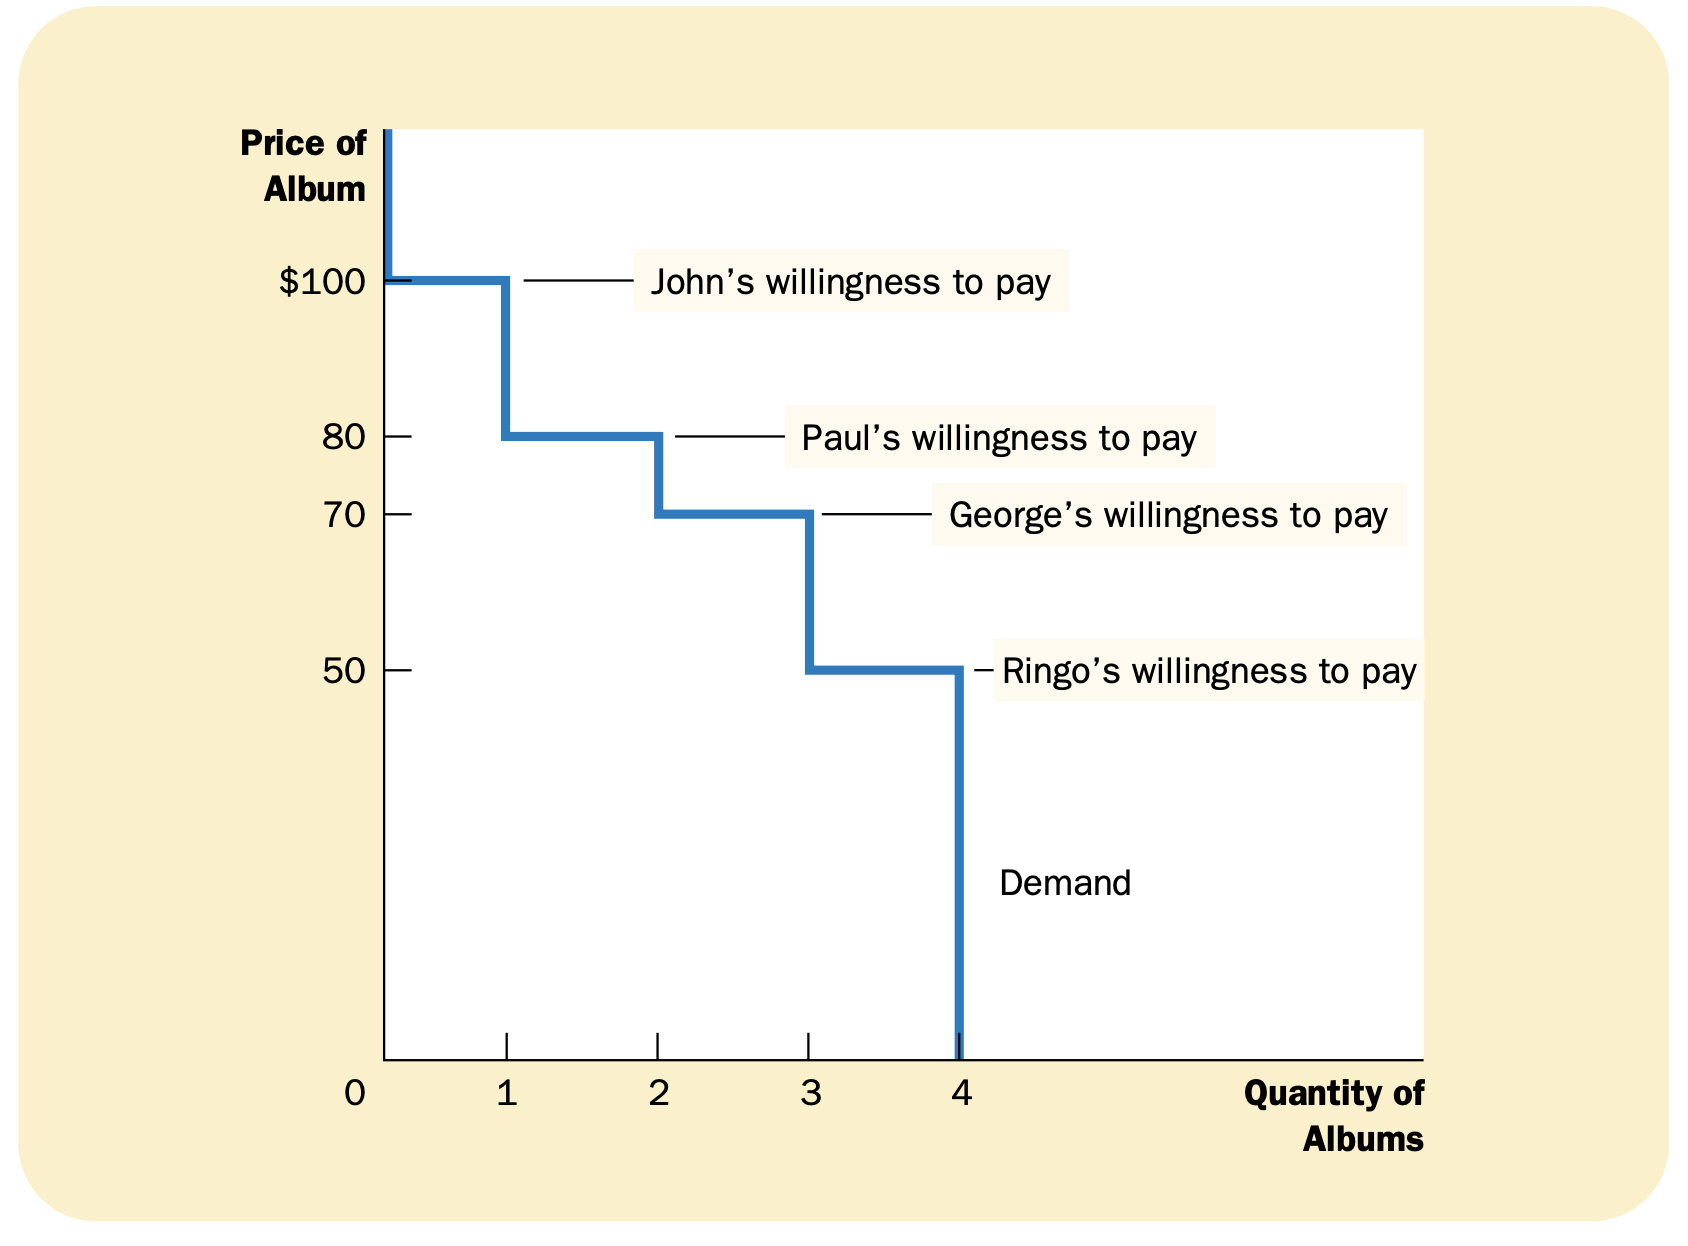
\includegraphics[width=\textwidth]{pics/willingness-to-pay}
  \caption{支付意愿}
  \label{fig:willingness-to-pay}
\end{figure}

\begin{figure}[!ht]
  \centering
  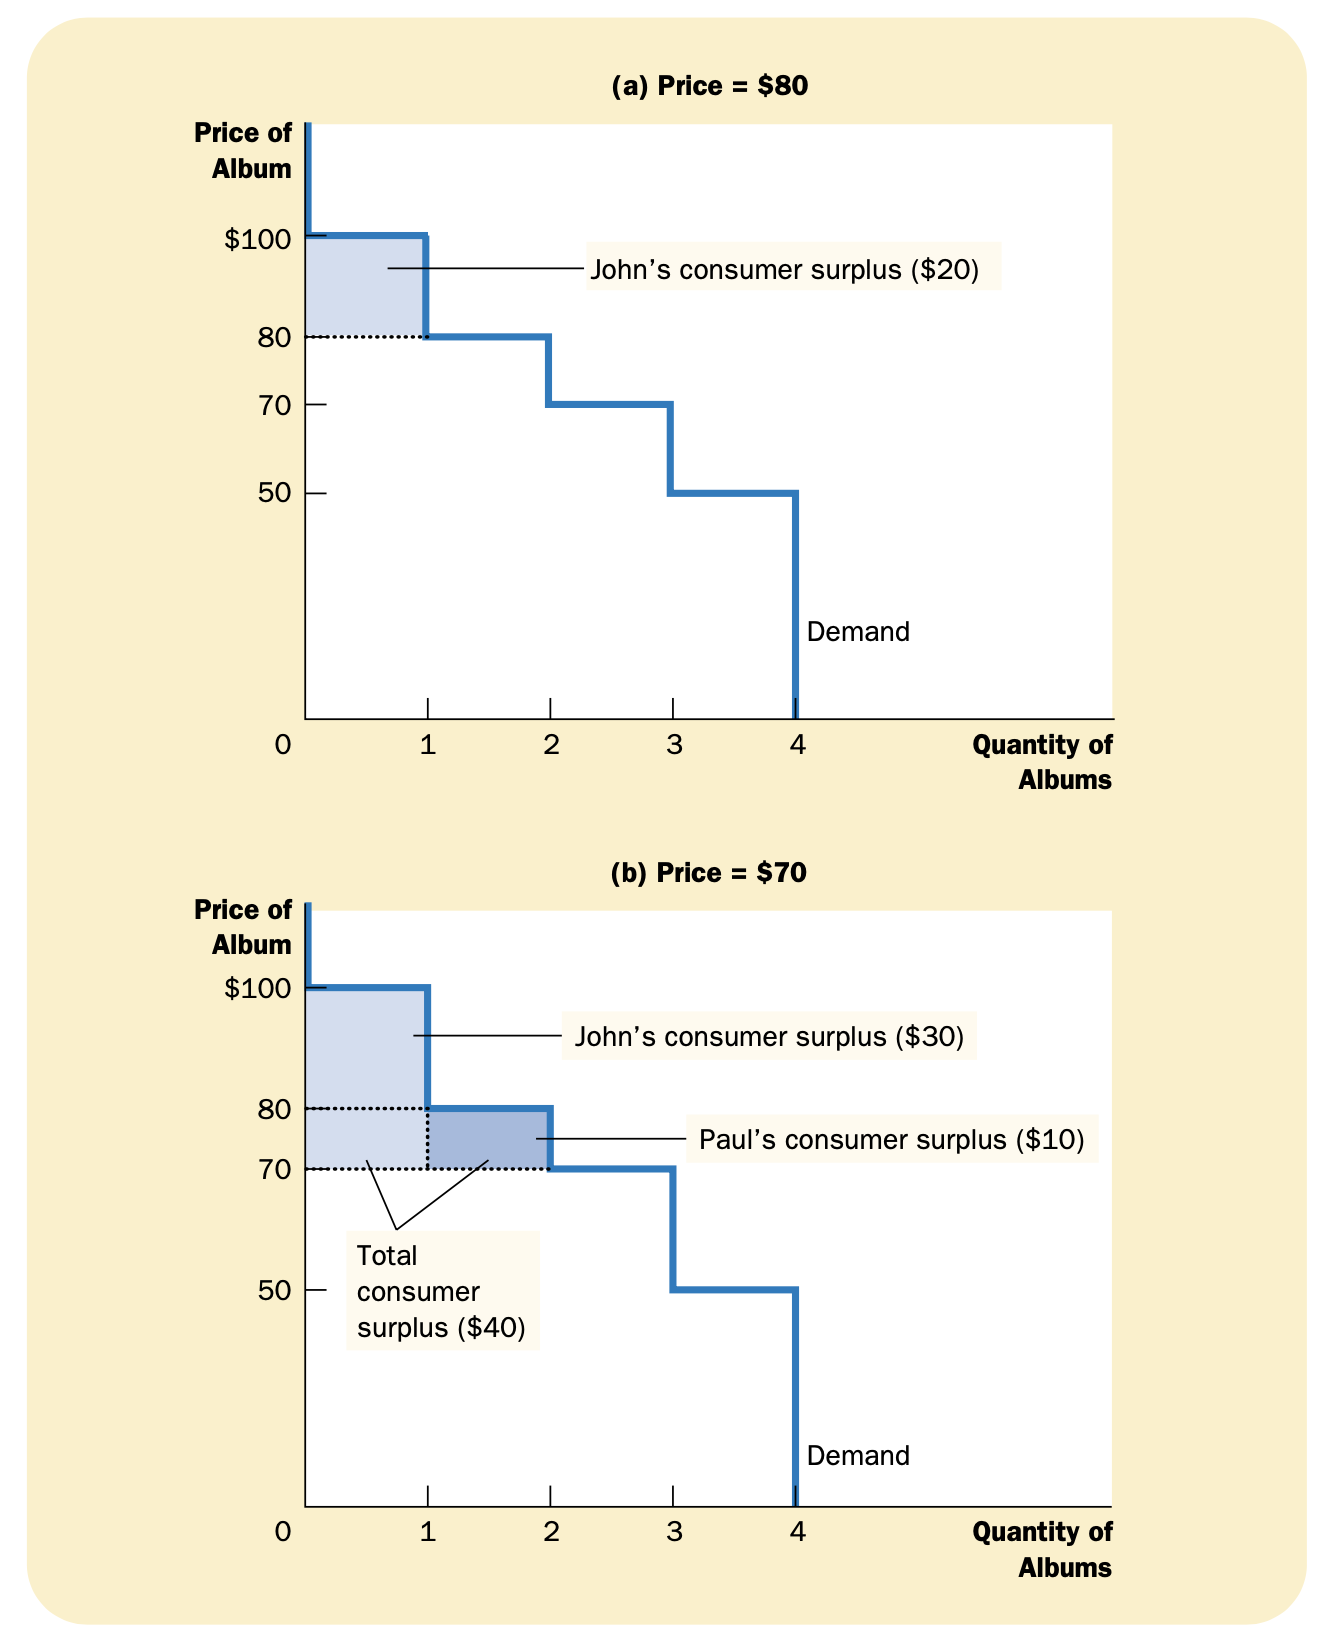
\includegraphics[width=\textwidth]{pics/consumer-surplus}
  \caption{消费者剩余}
  \label{fig:consumer-surplus}
\end{figure}

图\ref{fig:willingness-to-pay}和\ref{fig:consumer-surplus}表明:
需求曲线以下和价格以上的面积衡量一个市场上的消费者剩余。


\subsection{价格降低如何增加消费者剩余}

\begin{figure}[H]
  \centering
  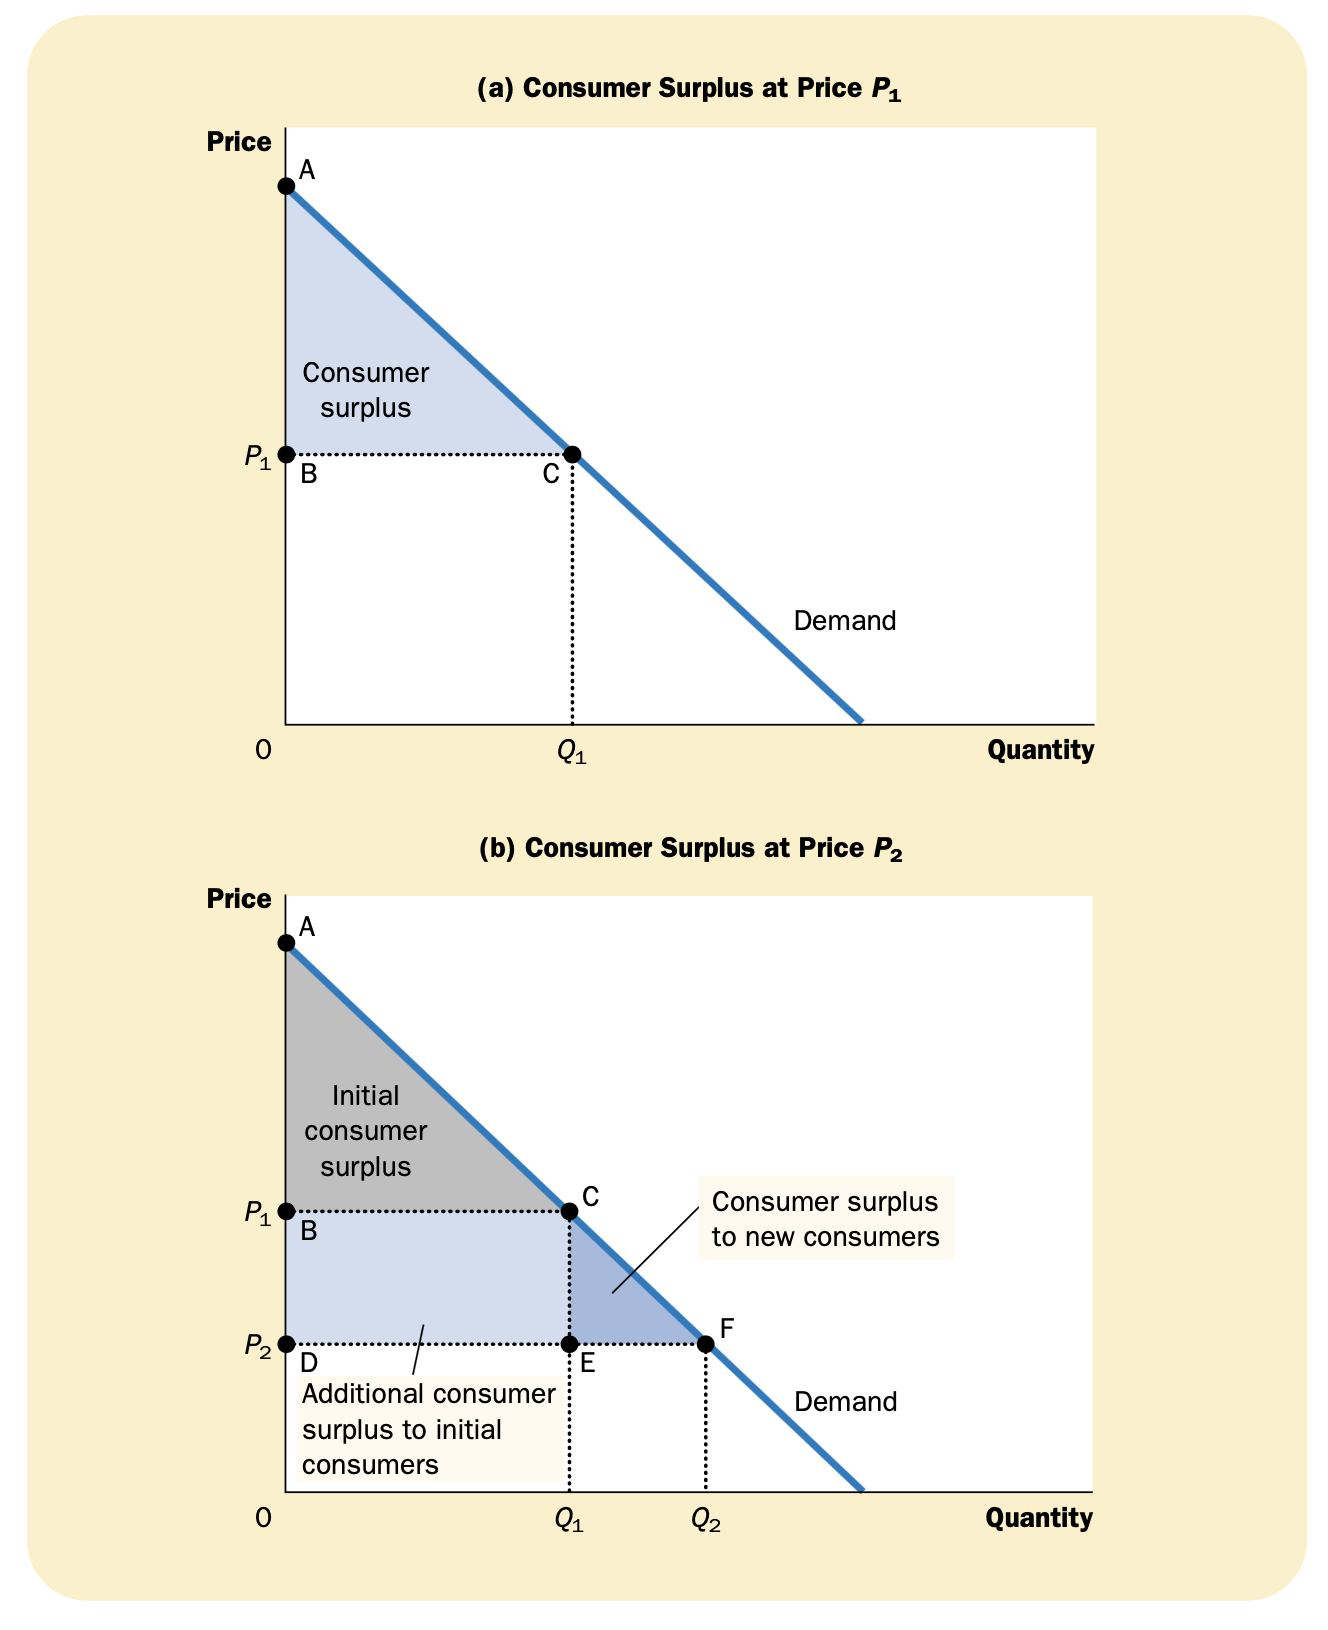
\includegraphics[width=\textwidth]{pics/consumer-surplus2}
  \caption{价格如何影响消费者剩余}
  \label{fig:consumer-surplus2}
\end{figure}


消费者剩余某种程度上不失为经济福利的一种好的衡量标准。

\section{生产者剩余}

\subsection{成本与销售意愿}

成本衡量卖者愿意出售其服务的意愿。

生产者剩余(producer surplus)是卖者得到的量减去其生产成本。
生产者剩余衡量卖者从参与市场中得到的利益。


\subsection{用供给曲线衡量生产者剩余}

边际卖者是如果价格再降低一点就首先离开市场的卖者。


\begin{figure}[!ht]
  \centering
  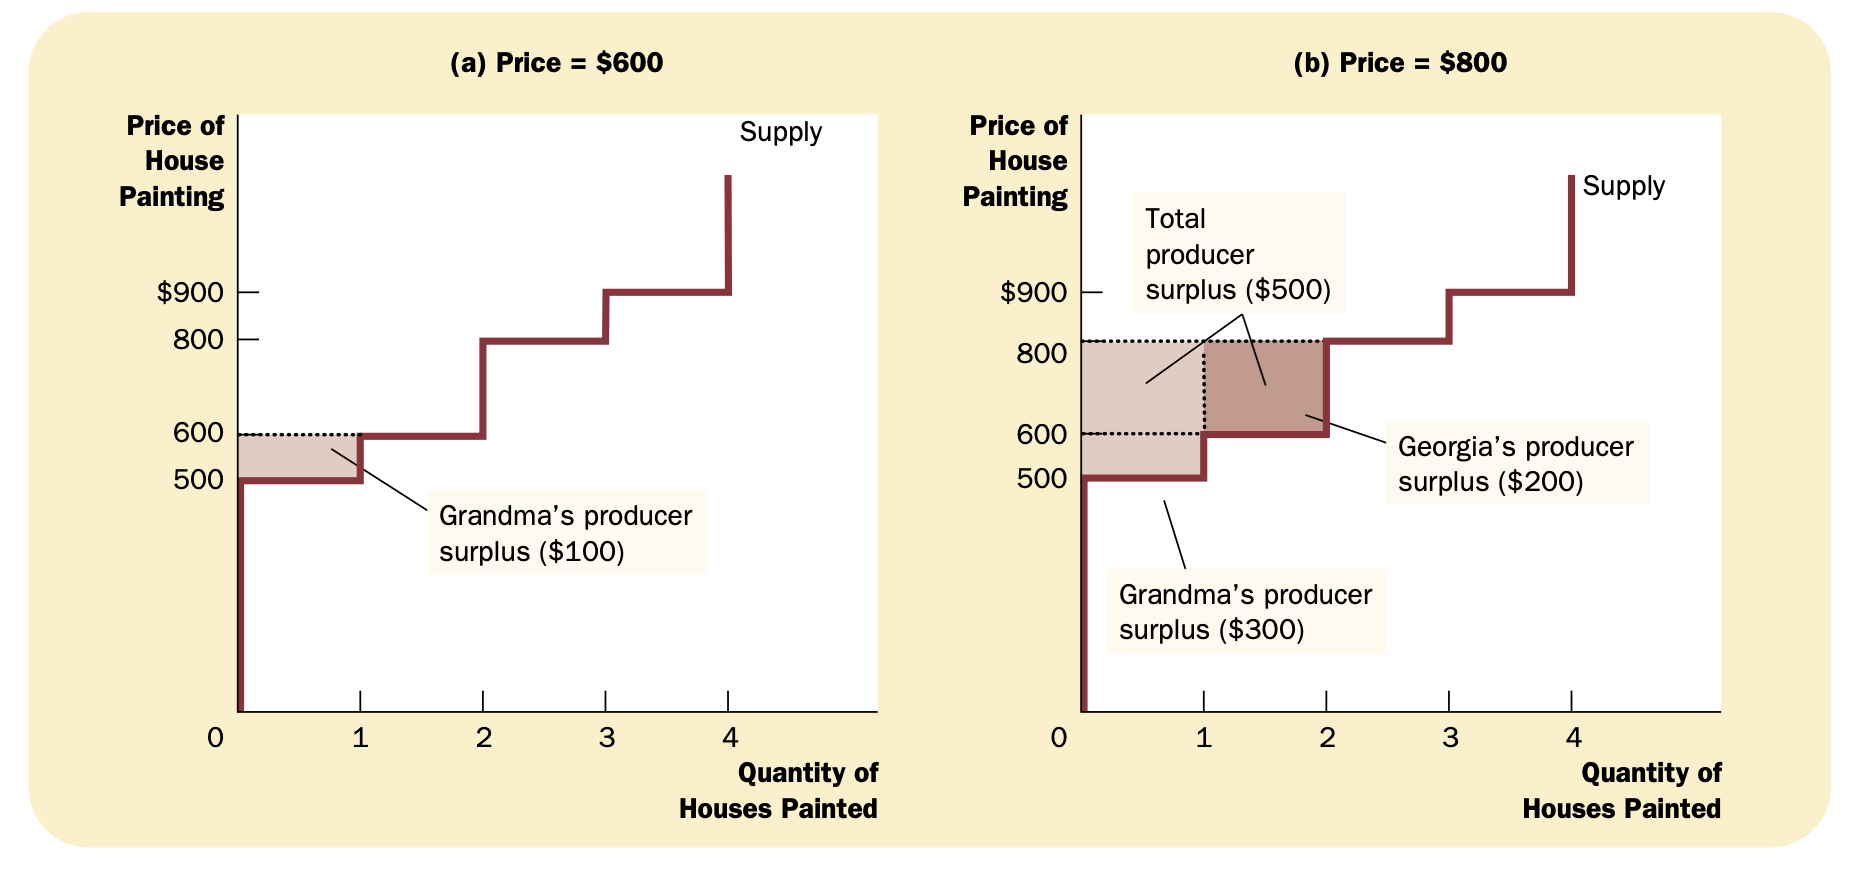
\includegraphics[width=\textwidth]{pics/producer-surplus}
  \caption{生产者剩余}
  \label{fig:producer-surplus}
\end{figure}

图\ref{fig:producer-surplus}表明:
价格之下和供给曲线以上的面积衡量一个市场上的生产者剩余。


\subsection{价格上升如何增加生产者剩余}

\begin{figure}[H]
  \centering
  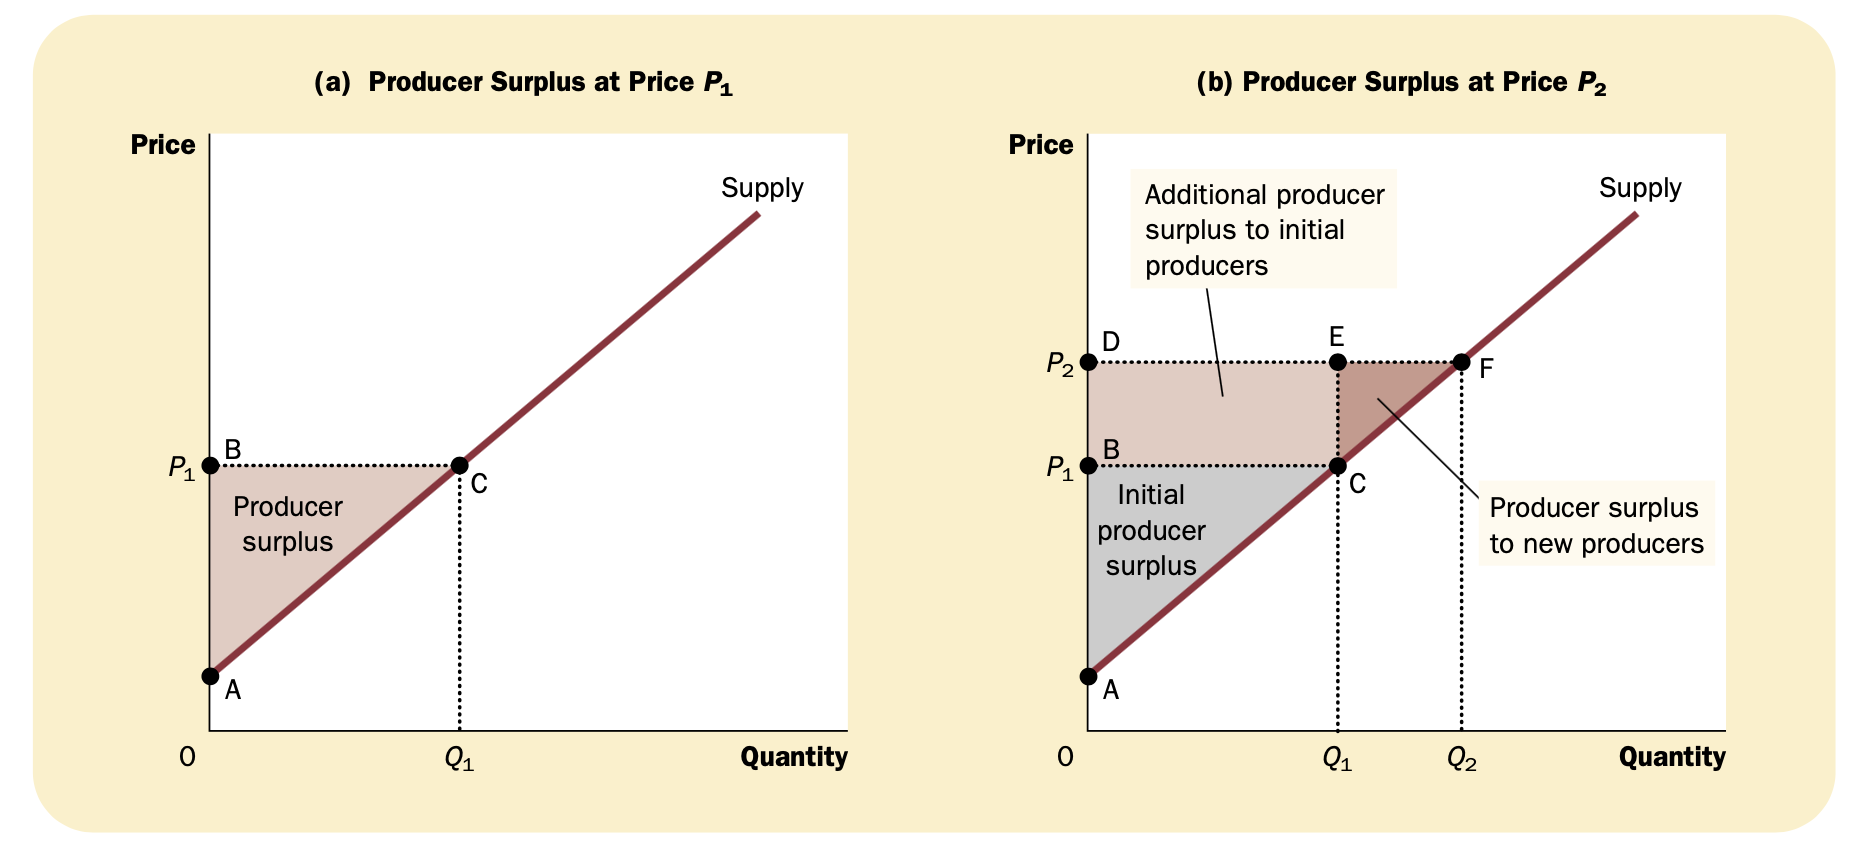
\includegraphics[width=\textwidth]{pics/producer-surplus2}
  \caption{价格上升如何增加生产者剩余}
  \label{fig:producer-surplus2}
\end{figure}


生产者剩余量某种程度上可以用来衡量卖者的福利。


\section{市场效率}



如何衡量社会的经济福利?
一种可能的衡量指标是消费者剩余与生产者剩余的总和,
我们称之为总剩余。


\begin{equation}
  \text{消费者剩余} = \text{买者的评价} - \text{买者支付的量}
\end{equation}
\begin{equation}
  \text{生产者剩余} = \text{卖者得到的量} - \text{卖者的成本}
\end{equation}

因为:
\begin{equation}
  \text{买者支付的量} = text{卖者得到的量}
\end{equation}

所以:
\begin{equation}
  \text{总剩余} = \text{买者的评价} - \text{卖者的成本}
\end{equation}


如果资源配置使总剩余量最大化,
我们可以说,
这种配置是\keyword{有效率}的。
如果一种配置是无效率的,
那么,买者和卖者之间交易的一些潜在的利益就还没有实现。
例如,如果一种物品不是由成本最低的卖者生产的,
配置就是无效率的,
在这种情况下,
将生产从高成本生产者转给低成本生产者就会降低卖者的总成本并增加总剩余。
同样,
如果一种物品不是对这种评价最高的买者消费,
配置也是无效率的。
在这种情况下,将物品的消费从评价低的买者转给评价高的买者就会增加总剩余量。


平等:市场上的各个买者与卖者是否有相似的经济福利水平。


在本质上,
从市场贸易中获得的利益就像一块要在市场参与者间分配蛋糕。
效率问题涉及的蛋糕是否尽可能地做大。
平等问题涉及的是如何把蛋糕切成小块,
以及如何在社会成员中进行分配。




\begin{figure}[!ht]
  \centering
  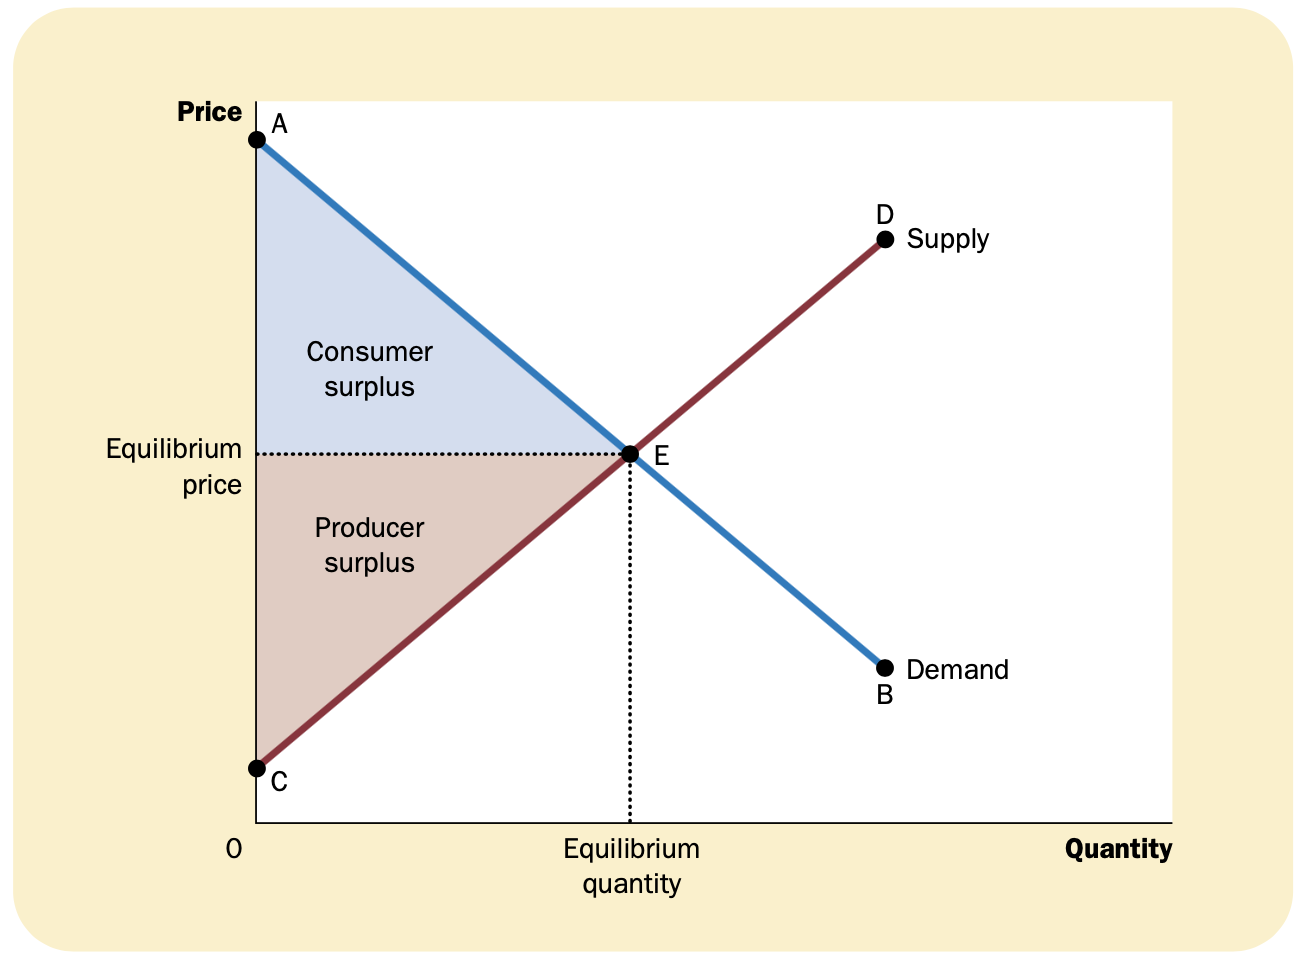
\includegraphics{pics/market-equilibrium}
  \caption{市场均衡时的消费者剩余与生产者剩余}
  \label{fig:market-equilibrium}
\end{figure}

\begin{figure}[!ht]
  \centering
  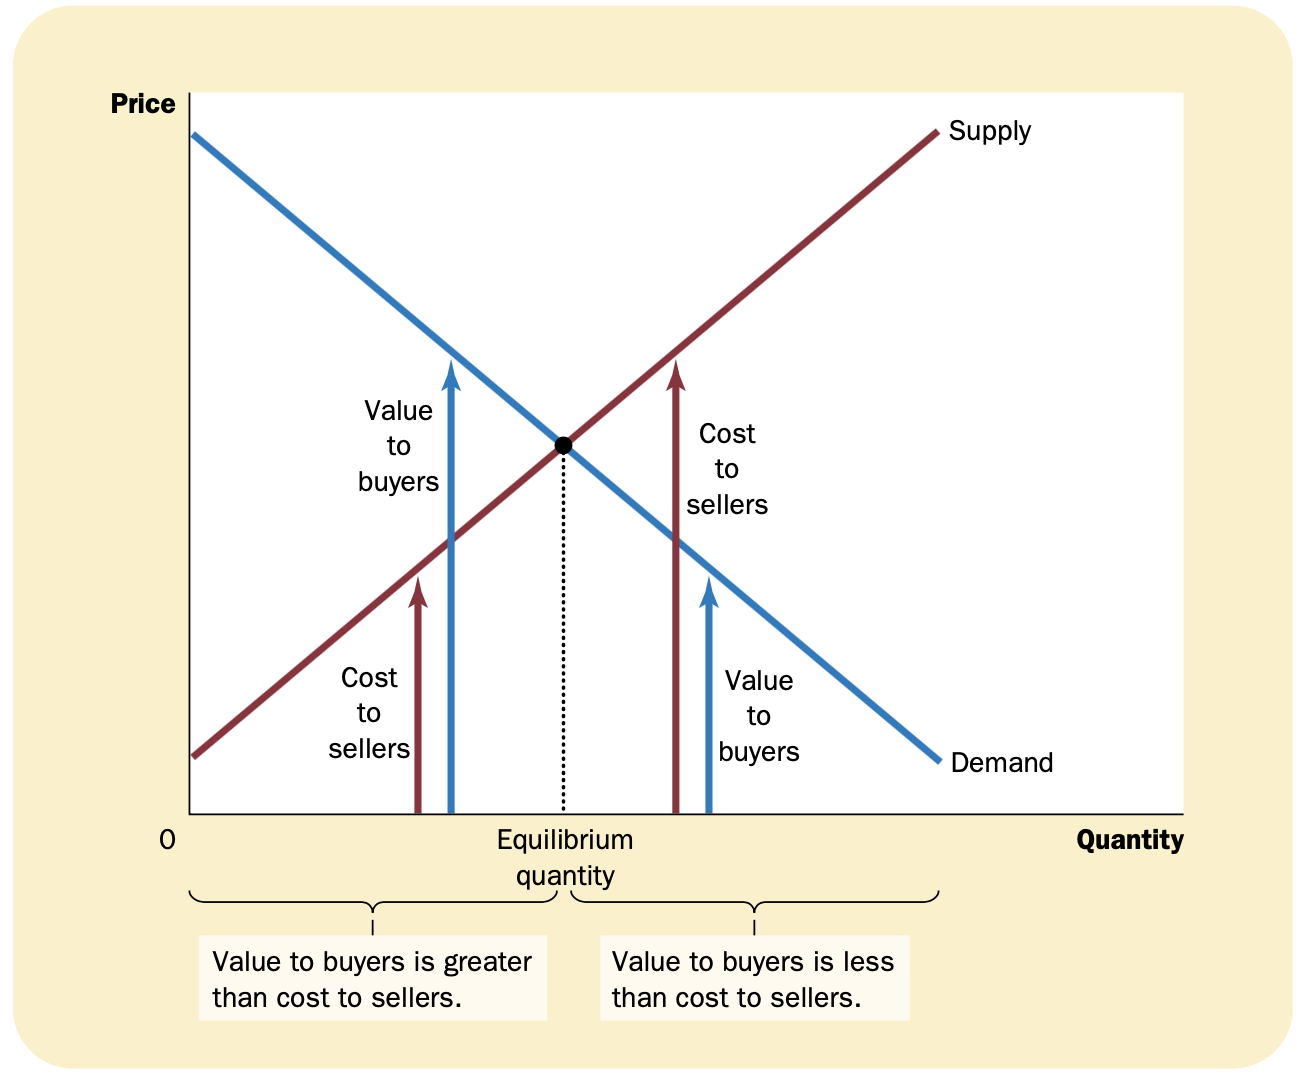
\includegraphics{pics/market-equilibrium2}
  \caption{均衡数量的效率}
  \label{fig:market-equilibrium2}
\end{figure}


从图\ref{fig:market-equilibrium}和\ref{fig:market-equilibrium2}可得出如下结论:
\begin{itemize}
\item 自由市场把物品的供给分配给对这些物品评价高的买者,这种评价用买者的支付意愿来衡量。
\item 自由市场将物品的需求分配给能够以最低成本生产这些物品的卖者。
\item 自由市场生产出使消费者剩余和生产者剩余的总和最大化的物品量。
\end{itemize}


\section{结论}

为了得出市场有效率的结论,
我们做出了一些关于市场如何运行的假设。
当这些假设不成立时,
关于市场均衡有效率的结论可能就不再正确了。


这些假设中有两个最重要的假设:
\begin{itemize}
\item 市场时完全竞争的。
\item 市场结果只影响参与市场的买者和卖者。
\end{itemize}


在现实世界中,在一些市场上,某个单个买者或者卖者(或一小群买者或卖者)可以控制市场价格。
这种影响价格的能力被称为\keyword{市场势力}。

在现实世界中,买者和卖者的决策有时会影响那些根本不参与市场的人。
污染是市场结果影响市场参与者以外的人的一个典型例子。
市场的这种副作用被称为\keyword{外部性}。

市场势力和外部性是一种被称为\keyword{市场失灵}的普遍现象的例子,
市场失灵是指一些不受管制的市场不能有效地配置资源。
当出现市场失灵时,公共政策有可能纠正这些问题并提高经济效率。

% 
\chapter{赋税的代价}


% \listoftables
% \listoffigures


\backmatter
\bibliographystyle{plainnat}
\bibliography{tex}
\end{document}
